\documentclass[11pt]{article}

% ---------------- Packages ----------------
\usepackage[a4paper,margin=1in]{geometry}
\usepackage{amsmath,amssymb}
\usepackage{booktabs}
\usepackage{array}
\usepackage{tabularx}
\usepackage{longtable}
\usepackage{enumitem}
\usepackage{graphicx}
\usepackage{caption}
\usepackage{subcaption}
\usepackage{float}
\usepackage{tikz}
\usetikzlibrary{arrows.meta,positioning}
\usepackage{pdflscape}
\usepackage{xcolor}
\usepackage[colorlinks=true,linkcolor=blue,citecolor=blue,urlcolor=blue]{hyperref}
\usepackage[activate={true,nocompatibility},final,tracking=true,kerning=true,spacing=true,factor=1100,stretch=10,shrink=10,expansion=false,protrusion=true]{microtype}
\usepackage{setspace}
\usepackage{titlesec}
\usepackage{fancyhdr}
\usepackage{parskip}
\usepackage{url}
\usepackage{xspace}
\usepackage{authblk}
\usepackage[numbers,sort&compress]{natbib}

\emergencystretch=3em
\graphicspath{{../data/results/run_20260526_v11_dct1_phospho_mediation/figures/v11/}{figures_v4/}{figures_osd462/}}
\setlist[itemize]{leftmargin=1.5em,itemsep=0.2em,topsep=0.25em}
\setlist[enumerate]{leftmargin=1.5em,itemsep=0.2em,topsep=0.25em}
\titleformat{\section}{\Large\bfseries}{\thesection}{0.8em}{}
\titleformat{\subsection}{\large\bfseries}{\thesubsection}{0.8em}{}
\titleformat{\subsubsection}{\normalsize\bfseries\itshape}{\thesubsubsection}{0.6em}{}

\pagestyle{fancy}
\fancyhf{}
\fancyhead[L]{\small Layer-resolved spaceflight kidney multi-omics}
\fancyhead[R]{\small \thepage}
\renewcommand{\headrulewidth}{0.4pt}

\newcommand{\code}[1]{\texttt{#1}}
\newcommand{\gene}[1]{\textit{#1}}
\newcommand{\RRRM}{RRRM-2\xspace}
\newcommand{\ISS}{ISS terminal\xspace}
\newcommand{\LAR}{live animal return\xspace}
\newcommand{\OSD}{OSDR\xspace}
\newcolumntype{Y}{>{\raggedright\arraybackslash}X}

\title{\textbf{Broad distal-nephron phosphoregulatory suppression in the spaceflight kidney}\\[0.35em]
\large Cross-cohort RNA recurrence and matched mouse-kidney multi-omics resolve the transporter phenotype beyond the NCC/DCT1 axis}
\author{Ibrahim Shahid}
\affil{Independent research manuscript}
\date{Draft, May 2026}

\begin{document}
\maketitle

\begin{abstract}
\noindent
Spaceflight dephosphorylates the sodium-chloride cotransporter NCC and its WNK--SPAK/OSR1 regulatory kinases in the kidney, but whether the accompanying transcriptomic response reflects, contradicts, or simply misses that endpoint had not been resolved. Analyzing public mouse kidney RNA-seq, TMT protein, and phosphoproteomic datasets (RRRM-2/OSD-771, OSD-513, OSD-253, and matched RR-10/OSD-462) against external DCT1/DCT2 single-nucleus, perturbation, spatial, and human-urine references, we show that the three layers disagree: a recurrent bulk-RNA remodeling response does not propagate to protein abundance, and the transporter phenotype is carried at regulatory phosphorylation---where it extends across the distal nephron more widely than the canonical NCC/DCT1 axis.

Across independent RNA cohorts, flight raised matrix/endothelial remodeling and lowered DCT/NCC-WNK transport scores; remodeling recurred robustly in a five-cohort meta-analysis ($p=7.0\times10^{-4}$), while transport suppression was more cohort-dependent and resolved most clearly at phosphorylation. In matched OSD-462 multi-omics the RNA program did not reach protein: RNA and protein flight effects were decoupled at genome scale (Spearman $-0.034$, the loose coupling expected for bulk tissue), and the one curated set with a null-tested protein effect, matrix/ECM, was inverted rather than concordant. Total NCC and related protein abundance stayed flat while NCC/SPAK/WNK regulatory phosphosites fell, and an unbiased kinome-wide screen independently recovered WNK1/WNK3 suppression from the full phosphosite background.

Ranking the parent genes of flight-suppressed phosphosites against the DCT1/DCT2 prior placed the suppression at distal-nephron subtype-prior extremes, most robustly in an aldosterone-sensitive DCT2/CNT--leaning bin that survived an observability-matched parent-gene permutation and parent-protein normalization. This broadens the spaceflight distal-nephron phenotype from a narrow NCC/DCT1 event toward coupled sodium, potassium, and calcium handling across the aldosterone-sensitive segment, and external perturbation and spatial references nominated DCT-adjacent remodeling neighborhoods as the spatial hypothesis to test.

The spaceflight kidney transcriptome is therefore a tissue-context readout that does not by itself report transporter state; DCT-subtype-resolved or spatial phosphoproteomics, not additional bulk transcriptomics, is the highest-priority next experiment and the one that can localize the broadened distal-nephron suppression.
\end{abstract}

\vspace{0.3em}
\noindent\textbf{Keywords:} spaceflight kidney; mouse kidney; distal convoluted tubule; NCC; SLC12A3; WNK; SPAK/OSR1; phosphoproteomics; DCT subtype prior; RNA-protein mismatch; OSD-462; RR-10.

\clearpage
\tableofcontents
\clearpage

% =====================================================================
\section{Introduction}

Kidney risk has long been part of human spaceflight medicine, framed initially around altered calcium balance and the elevated renal stone risk carried by astronauts during and after flight \citep{cockett1962astronautical,pietrzyk2007renal,smith2014men}. Its proximate cause is mechanical. In microgravity the loss of a gravitational gradient produces a cephalad fluid shift that redistributes roughly two litres of blood and interstitial fluid from the lower body toward the thorax and head, forcing thoracic vascular beds to accommodate the displaced volume \citep{spacekidney2023}. The kidney sits directly downstream of this redistribution: altered central volume sensing changes the renal handling of sodium and water---reduced urinary sodium, sodium retention, and shifts in glomerular filtration and urinary albumin excretion \citep{christensen2001renal,drummer2001water}---and these functional changes are accompanied by structural ones, with kidneys examined after real or simulated microgravity showing glomerular atrophy, interstitial edema, and degeneration of renal tubular cells \citep{liakopoulos2012kidney}. More recent rodent work has moved the emphasis from stone physiology toward active tubular dysfunction, describing renal tubulopathy, interstitial and vascular remodeling, mitochondrial and oxidative-stress responses, and altered solute handling \citep{afshinnekoo2020fundamental,daSilveira2020comprehensive,chouker2025impact}, much of it enabled by rodent studies that profile kidney tissue directly across transcriptomic, proteomic, phosphoproteomic, and histologic layers.

The Cosmic Kidney Disease study integrated human and rodent spaceflight datasets with microgravity and galactic-cosmic-radiation models to define a multi-omic picture of spaceflight-induced renal dysfunction, and reported dephosphorylation of the sodium-chloride cotransporter NCC (\gene{Slc12a3}) and related distal-nephron transport machinery alongside distal convoluted tubule (DCT) remodeling \citep{siew2024cosmic}. That work established the dephosphorylation endpoint; it did not resolve whether the same transporter phenotype is reflected, or contradicted, across the transcriptomic and protein-abundance layers, nor how far across the distal-nephron subtype map the suppressed phosphoregulation extends. The mouse kidney omics in that study derive from Rodent Research-10, deposited as OSD-462: kidney RNA-seq, TMT proteomics, and phosphoproteomics measured on the same flight and ground-control mice (B6129SF2/J; $n=20$ in the matched flight-versus-control comparison). We analyze OSD-462 together with independent mouse kidney RNA-seq cohorts to define the flight RNA signature, compare RNA against protein abundance across the remodeling and distal-nephron programs, quantify NCC/SPAK/WNK regulatory phosphosite changes, and rank the parent genes of suppressed phosphosites against an external DCT1/DCT2 subtype reference.

NCC reabsorbs sodium and chloride in the distal convoluted tubule, and its activity is governed less by its abundance than by phosphorylation of an N-terminal regulatory cluster: the WNK kinases activate the Ste20-type kinases SPAK and OSR1, which phosphorylate this cluster to switch the transporter on \citep{vitari2005wnk,moriguchi2005wnk,richardson2008wnk,pachecoalvarez2006ncc} (Fig.~\ref{fig:axis}). Suppression of these regulatory phosphosites therefore lowers NCC activation largely independently of transporter protein level, with downstream effects on distal sodium-chloride balance and on the coupled potassium, calcium, and magnesium handling of the segment. Loss of NCC activity is the molecular lesion of Gitelman syndrome---salt wasting with volume contraction and a tendency to hypotension, hypokalemia, and hypomagnesemia \citep{gamba2005cct}---so a spaceflight-induced reduction in NCC activation would be expected to perturb fluid and electrolyte balance in microgravity, which makes the regulatory phosphorylation layer the physiologically decisive one. The DCT is itself heterogeneous: DCT1 carries this WNK--SPAK/OSR1--NCC electroneutral NaCl-reabsorption axis, whereas the later DCT2/CNT transition adds aldosterone-sensitive sodium transport and the principal calcium/magnesium machinery (\gene{Trpv5}, \gene{Calb1}) \citep{loffing2001distal}. Which subtype a suppressed phosphosite belongs to is therefore biologically informative, and motivates the DCT1/DCT2 prior introduced below.

\begin{figure}[t]
\centering
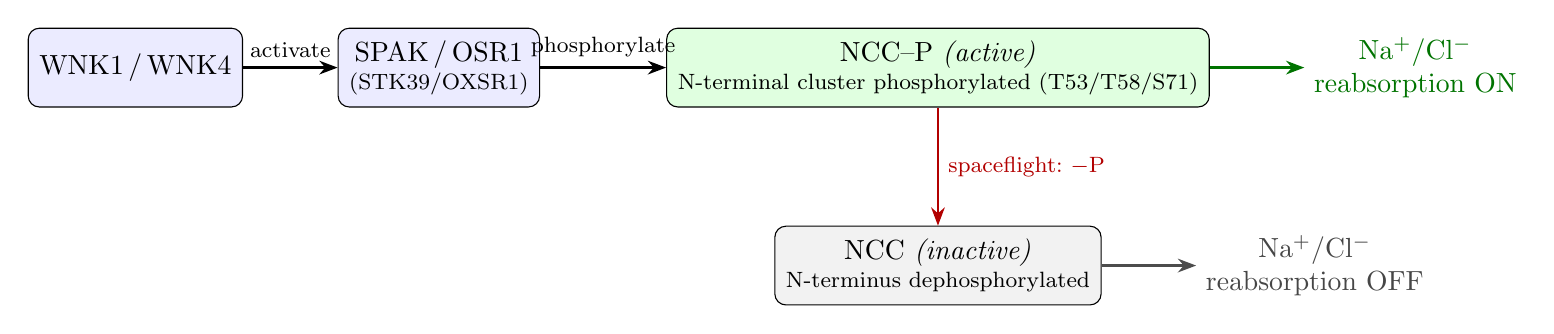
\begin{tikzpicture}[>=Stealth, node distance=12mm,
  box/.style={draw, rounded corners, align=center, minimum height=10mm, inner sep=4pt}]
\node[box, fill=blue!8] (wnk) {WNK1\,/\,WNK4};
\node[box, fill=blue!8, right=of wnk] (spak) {SPAK\,/\,OSR1\\[-2pt]{\footnotesize (STK39/OXSR1)}};
\node[box, fill=green!12, right=16mm of spak] (ncc) {NCC--P \emph{(active)}\\[-2pt]{\footnotesize N-terminal cluster phosphorylated (T53/T58/S71)}};
\node[right=of ncc, align=center, text=green!45!black] (na) {Na$^+$/Cl$^-$\\reabsorption ON};
\node[box, fill=gray!10, below=15mm of ncc] (ncc0) {NCC \emph{(inactive)}\\[-2pt]{\footnotesize N-terminus dephosphorylated}};
\node[right=of ncc0, align=center, text=gray!55!black] (na0) {Na$^+$/Cl$^-$\\reabsorption OFF};
\draw[->,thick] (wnk) -- node[above,font=\footnotesize]{activate} (spak);
\draw[->,thick] (spak) -- node[above,font=\footnotesize]{phosphorylate} (ncc);
\draw[->,thick,green!45!black] (ncc) -- (na);
\draw[->,thick,gray!60!black] (ncc0) -- (na0);
\draw[->,red!70!black,thick] (ncc) -- node[right,font=\footnotesize]{spaceflight: $-$P} (ncc0);
\end{tikzpicture}
\caption{\textbf{The WNK--SPAK/OSR1--NCC regulatory axis and its activation state.} WNK kinases activate SPAK and OSR1, which phosphorylate the N-terminal regulatory cluster of NCC; phosphorylated NCC is active and drives distal sodium-chloride reabsorption (top), whereas dephosphorylated NCC is inactive (bottom). In OSD-462 spaceflight kidney this regulatory phosphorylation is suppressed while total NCC protein abundance is unchanged, shifting NCC toward the inactive state---so the transporter-regulatory deficit is visible at the phosphorylation layer, not at protein abundance.}
\label{fig:axis}
\end{figure}

This is what bulk kidney RNA-seq cannot settle on its own. A whole-kidney transcriptome reports which cell types are present as much as how each cell regulates transport, so a recurring pattern of higher matrix/endothelial and lower DCT/NCC-WNK signal is equally compatible with DCT transcriptional suppression, DCT segment loss, or dilution by expanding interstitial and endothelial compartments---and, because transcript and protein abundance are only loosely coupled in tissue \citep{liu2016dependency}, such a pattern need not correspond to any change in transporter protein or its activation state. Resolving the transporter phenotype therefore requires the matched protein and phosphorylation layers, read against a subtype reference that assigns each suppressed phosphosite to a part of the distal nephron. We accordingly combine cross-cohort RNA recurrence with OSD-462 protein and phosphoprotein contrasts and an external native DCT1/DCT2 single-nucleus reference.

Three questions follow, each posed at the layer where it can be answered. Does the flight RNA response reproduce across independent kidney cohorts as a tissue-context program of matrix/endothelial remodeling with lower DCT/NCC-WNK transport? When the same animals are read at protein abundance, does that RNA program propagate, or does the transporter signal instead localize to NCC/SPAK/WNK regulatory phosphorylation? And do the parent genes of flight-suppressed phosphosites concentrate at the extremes of the distal-nephron subtype prior, marking which DCT1- and DCT2/CNT-associated programs lose regulatory phosphorylation? We answer them with within-study gene-set scoring and cross-cohort pathway-vector recurrence, OSD-462 protein and phosphosite contrasts with targeted and kinome-wide kinase-substrate enrichment, and native DCT1/DCT2 parent-gene enrichment, supported by composition-aware, perturbation-reference, spatial-reference, and human fluid-axis analyses.

Read this way, the spaceflight kidney transporter phenotype is not a transcriptional or abundance program but a regulatory-phosphorylation one, and its reach across the distal nephron is wider than the canonical NCC/DCT1 axis. The parent genes of flight-suppressed phosphosites are enriched at distal-nephron subtype-prior extremes, most robustly at the aldosterone-sensitive DCT2/CNT--leaning end where the SGK1--NEDD4L--ENaC axis and the principal calcium-handling machinery are regulated. This reframes the spaceflight distal-nephron phenotype from a narrow NCC/DCT1 event toward a broader phosphoregulatory suppression of the aldosterone-sensitive distal nephron---a hypothesis that the matched layers raise and that segment-resolved phosphoproteomics can test directly.

% =====================================================================
\section{Methods}

\subsection{Datasets and study roles}

The datasets were assigned fixed roles---anchor, recurrence, context, and external reference---so that each analysis drew on data at its appropriate resolution. RRRM-2/OSD-771 served as the primary RNA-seq cohort because its design is the richest: it spans young and old female C57BL/6NTac mice across ISS terminal dissection, live animal return, flight, habitat ground control, vivarium, and basal contexts, supporting within-mission flight-versus-habitat-control contrasts and age stratification that the other cohorts do not. Primary flight contrasts compared flight with habitat ground control within mission arm. OSD-513 provided the independent flight cohort used to test whether the RRRM-2 RNA pattern recurs, and was deliberately kept separate so that recurrence is assessed on data not used to define the pattern. OSD-253 served as a strain and mechanism-context cohort because it includes C57BL/6J and C3H/HeJ mice and more complex ground-control definitions. OSD-462/RR-10 supplied kidney RNA-seq, TMT proteomics, and phosphoproteomics for flight and ground-control samples. The cross-cohort recurrence meta-analysis additionally drew on OSD-102 and OSD-163 as independent OSDR mouse-kidney flight cohorts (C57BL/6J and BALB/c-background strains, respectively), widening the strain and mission span over which remodeling recurrence is assessed. % CONFIRM OSD-102/OSD-163 accessions, strains, and that both are kidney RNA-seq before finalizing.

GSE228367 was used as an external native DCT1/DCT2 single-nucleus RNA reference \citep{su2024dct}. PXD001729 was used as a cultured DCT-lineage phosphoproteomic reference from mpkDCT cells stimulated with dDAVP/vasopressin \citep{cheng2015mpkdct}. GSE269622 and GSE269719 were used as external kidney ischemia-reperfusion injury (IRI) spatial reference datasets, with Visium supporting whole-transcriptome pathway projection and Xenium supporting annotation context \citep{spatial2025iri}. Tabula Muris Senis kidney was used only as an external aging reference \citep{tabula2020}.

\subsection{RNA preprocessing and gene-set scoring}

Primary RRRM-2 analyses used the project residualized expression matrix and matched metadata generated by the repository preprocessing pipeline. External cohorts were analyzed within study rather than pooled at raw-expression level, because spaceflight datasets differ in mission, strain, sex, preservation, sequencing, and metadata. Differential-expression and preprocessing resources followed standard RNA-seq/Bioconductor practices \citep{ritchie2015limma,love2014deseq2,robinson2010edger}.

Curated gene sets summarized ECM organization, integrin/cell adhesion, MMP/ADAM proteolysis, endothelial and stromal context, DCT/NCC-WNK transport, broad tubular transport, TLR4/innate signaling, macrophage/inflammatory context, S1P/S1PR3 signaling, oxidative stress/NRF2, and preservation/sample-stress response. These were literature-curated panels of canonical pathway members rather than imported ontology terms, chosen to summarize the spaceflight remodeling and distal-transport axes at interpretable resolution; gene symbols were resolved against an Ensembl-backed identifier map, and the frozen member lists, pathway-family labels, leave-one-family recurrence check, and paired pathway bootstrap are emitted with the v11 run artifacts. Gene-set scores were computed separately within each study. For gene $g$, sample $i$, study $c$, and curated gene set $G_k$, the sample-level score is defined as
\[
Z_{g i}^{(c)}=\frac{X_{g i}^{(c)}-\bar{X}_{g\cdot}^{(c)}}{s_{g\cdot}^{(c)}}, \qquad
S_{i k}^{(c)}=\frac{1}{|G_k\cap U_c|}\sum_{g\in G_k\cap U_c} Z_{g i}^{(c)},
\]
where $X_{g i}^{(c)}$ is the processed expression value, $\bar{X}_{g\cdot}^{(c)}$ and $s_{g\cdot}^{(c)}$ are the within-study mean and standard deviation for gene $g$, and $U_c$ is the set of genes observed in study $c$. Thus, scores are within-study mean standardized expression of observed member genes, not pooled cross-study expression values---a per-sample standardized-mean gene-set score.

Flight effects were computed as Space Flight minus Ground Control within the relevant study arm or comparison group:
\[
\Delta_{k r}^{(c)}=\frac{1}{n_{\mathrm{FLT},r}}\sum_{i\in \mathrm{FLT},r}S_{ik}^{(c)}
-\frac{1}{n_{\mathrm{GC},r}}\sum_{i\in \mathrm{GC},r}S_{ik}^{(c)},
\]
where $r$ indexes the arm, age, or comparison stratum. In RRRM-2, primary contrasts compared flight with habitat ground control within ISS terminal and live-return arms. When age-specific effects were needed, young and old strata were estimated separately; age-balanced arm summaries averaged the available age-specific flight-minus-control effects:
\[
\Delta_{k,\mathrm{arm}}^{(c)}=\frac{1}{|A|}\sum_{a\in A}\Delta_{k,\mathrm{arm},a}^{(c)}.
\]
The primary cross-cohort pathway vectors used within-study differences of means over shared gene-set features rather than a pooled multi-cohort regression. The ECM-DCT differential was computed as a compact scalar in which larger values indicate higher ECM/remodeling scores with lower DCT/NCC-WNK transport scores.

\subsection{Cross-cohort recurrence analysis}

Within each study, flight effects were computed as Space Flight minus Ground Control at gene-set or pathway level. RRRM-2 ISS terminal and live-return arm effects were computed separately. Cross-cohort recurrence was assessed by cosine similarity between pathway-effect vectors:
\[
\cos(\Delta^{A},\Delta^{B})=
\frac{\sum_{k}\Delta_{k}^{A}\Delta_{k}^{B}}
{\sqrt{\sum_k(\Delta_{k}^{A})^2}\sqrt{\sum_k(\Delta_{k}^{B})^2}}.
\]
The primary recurrence comparison used nine shared pathway features: apoptosis, calcium handling, DCT/NCC-WNK transport, ECM remodeling, fibrosis, inflammation, ion transport, lipid metabolism, and oxidative stress. Bootstrap confidence intervals used 2,000 resamples and permutation $p$ values used 5,000; the larger permutation count gives finer tail resolution for the small $p$ values, whereas interval coverage stabilizes at fewer resamples. In each bootstrap iteration, animals in the external cohort were resampled with replacement within flight and control strata, the external pathway-effect vector was recomputed, and the fixed RRRM-2 reference vector was reused. In each permutation, external-cohort flight/control labels were shuffled over the same samples, the external vector was recomputed, and the RRRM-2 direction was held fixed. Directional and two-sided absolute-tail permutation probabilities were calculated with a plus-one correction, for example $p=(1+\#\{\cos_{\mathrm{null}}\geq \cos_{\mathrm{obs}}\})/(1+B)$ for a positive directional test with $B$ permutations. Cosine values were interpreted against these bootstrap and permutation nulls rather than against a fixed cutoff: a value near zero indicates no shared pathway direction, and overlap of the bootstrap intervals---not the point estimates alone---determines whether two cohorts differ in recurrence strength.

OSD-513 was interpreted as the primary recurrence cohort; OSD-253 was interpreted as contextual because of control-scenario complexity. For sample-level plotting, the recurrent RNA score was defined from the RRRM-2 ISS terminal and OSD-513 pathway effects that agreed in direction. The RRRM-2 and OSD-513 effect vectors were unit-normalized, averaged, oriented so ECM/fibrosis features were positive, restricted to pathway directions shared by both cohorts, and renormalized to unit length. This shared-direction score retained apoptosis, DCT/NCC-WNK transport, ECM remodeling, fibrosis, and oxidative stress; calcium handling, inflammation, ion transport, and lipid metabolism were excluded from this scalar because they disagreed between cohorts or were broad sensitivity features. Each cohort's sample-by-pathway score matrix was standardized by pathway within cohort and projected onto those weights. Higher values correspond to stronger matrix/endothelial remodeling and lower DCT/NCC-WNK transport.

RRRM-2 also allowed a planned age-by-flight network question. Control-aging vectors were estimated as old ground control minus young ground control within arm. Bootstrap stability showed that primary module/pathway aging directions were not stable enough to support a main age-rewiring claim. Age-related and live-return analyses are therefore reported as secondary context rather than central results.

\subsection{Matched OSD-462 multi-omic analysis}

The OSD-462 analysis was specified before computing the protein and phosphoprotein flight effects. RNA recurrence was tested by comparing the OSD-462 RNA pathway-effect vector with the RRRM-2 ISS terminal RNA direction. OSD-462 RNA effects used the OSDR differential-expression table for Space Flight versus Ground Control.

Protein abundance was analyzed from scaled TMT signal-to-noise values. Non-positive values were treated as missing; in the quantified protein and phosphosite rows carried into the contrasts this affected a negligible fraction of channels (median and maximum per-channel missing fraction 0.0 across plexes and conditions in the emitted QC summary), so the rule had little effect on the retained data. Values were log$_2$ transformed and median-centered within TMT plex and channel to reduce sample-loading differences. Protein-level flight effects were computed as within-plex differences and then averaged across available plexes:
\[
Y_{r j p}=\log_2(\mathrm{SN}_{r j p})-\mathrm{median}_{r}\{\log_2(\mathrm{SN}_{r j p})\}, \qquad
\delta_{r p}=\bar{Y}_{r,\mathrm{FLT},p}-\bar{Y}_{r,\mathrm{GC},p}, \qquad
\delta_{r}=\frac{1}{|P_r|}\sum_{p\in P_r}\delta_{r p}.
\]
Here $r$ indexes protein rows, $j$ sample channels, and $p$ TMT plex. A row-level plex effect required at least two finite flight and two finite ground-control channels within that plex; otherwise that plex contribution was missing. The primary gene-level protein table required both plexes where possible and collapsed multiple protein rows per gene by peptide-count-weighted averaging. Peptide coverage was therefore used for filtering, row-to-gene weighting, and matched-null construction, not as a regression covariate in the protein-abundance contrast. Protein effects were estimated as log$_2$ within-plex flight-minus-control differences followed by gene-level aggregation rather than with a moderated linear model such as limma: with only two plexes and few channels, empirical-Bayes shrinkage adds little and the within-plex difference keeps the contrast transparent. Raw-workbook TMT QC summaries of channel medians and missingness are emitted for protein, single-position phosphosite, and composite phosphosite sheets with the v11 baseline artifacts.

Protein-abundance concordance was tested for curated matrix/ECM, DCT/NCC-WNK, TLR4/innate, and S1P gene sets against abundance- and peptide-count-matched random gene-set nulls. Phosphosite effects were estimated per site and evaluated for the WNK--SPAK/OSR1--NCC regulatory chain, with total NCC protein abundance used as a control for whether phosphosite changes reflected altered phosphorylation rather than transporter abundance. RRRM-2 network-prioritized genes were also tested for enrichment among OSD-462 protein- or phosphoprotein-changing genes as an exploratory negative-control layer.

To generalize the RNA--protein mismatch beyond the targeted endpoint sets, a cross-layer pathway matrix was generated for the 11 curated OSD-462 pathway panels. Curated pathway genes were matched case-insensitively to OSD-462 RNA pathway effects, gene-level protein flight effects, and parent-gene-level mean phosphosite flight effects. Direction calls used small effect thresholds to avoid treating near-zero averages as directional (RNA $|\Delta|<0.04$, protein and phosphosite $|\Delta|<0.02$). This matrix is descriptive, summarizing where curated pathway signals appear across molecular layers rather than testing the significance of individual genes or sites. To calibrate these descriptive direction calls into per-pathway layer assignments, three pathway statistics were tested against an abundance- and peptide-count-matched random-gene-set null ($n=10{,}000$ draws): the within-pathway ordinary-least-squares slope of protein effect on RNA effect, the mean protein effect signed by the RNA-pathway direction, and the fraction of pathway members with matching RNA and protein signs. Benjamini-Hochberg correction was applied within the 11-pathway family. Detectability robustness was assessed by extending the matched stratum with a per-gene missing-fraction bin and rerunning the same tests (\path{src/v11/rna_protein_propagation.py}, \path{src/v11/observability_audit.py}).

Phosphosite abundance was analyzed from scaled phosphoproteomic TMT signal-to-noise values using the same log$_2$ transformation and within-channel median centering. For each phosphosite $s$, unadjusted flight effects and nominal $p$ values were estimated by ordinary least squares across animal channels:
\[
Y_{s j}=\beta_{0s}+\beta_{Fs}\mathbf{1}(\mathrm{Flight}_j)+\beta_{Ps}\mathbf{1}(\mathrm{Plex2}_j)+\epsilon_{s j}.
\]
The plex term was included when finite values were present in both plexes and dropped when only one plex contributed. Sites required at least three finite flight and three finite ground-control values. The coefficient $\beta_{Fs}$ is the Space Flight minus Ground Control phosphosite effect. Two-sided $p$ values used the ordinary least-squares residual standard error and residual degrees of freedom, and Benjamini-Hochberg q values were computed across quantified sites for site-level summaries. Flight-suppressed phosphosites for the primary enrichment analysis were defined as $\hat{\beta}_{Fs}<0$ and nominal $p<0.05$.

\subsection{DCT1/DCT2 reference prior and phosphosite enrichment}

GSE228367 DCT1 and DCT2 nuclei from normal-potassium controls (18{,}881 DCT1 and 6{,}274 DCT2 nuclei across three replicates) were aggregated by subtype and replicate. Gene symbols were harmonized to OSD-462 phosphosite parent genes. For each gene, a DCT1 enrichment score was computed as the difference between mean DCT1 and DCT2 expression:
\[
D_g=\bar{E}_{g,\mathrm{DCT1}}-\bar{E}_{g,\mathrm{DCT2}}.
\]
A log-ratio with a small offset, $\log_2[(\bar{E}_{g,\mathrm{DCT1}}+0.01)/(\bar{E}_{g,\mathrm{DCT2}}+0.01)]$, was used for marker checks and binary DCT1-core summaries. DCT1 top-quartile/top-decile bins and DCT2-leaning low-DCT1-score quartile/decile bins were defined among genes detected in the DCT reference. As a post-hoc sanity check, known DCT markers were confirmed to fall on their expected side of the prior---DCT1-leaning \gene{Pvalb}, \gene{Trpm6}, \gene{Stk39}, and \gene{Wnk4}, and DCT2/CNT-associated \gene{Trpv5} and \gene{Calb1}---which confirmed prior orientation but did not feed back into or alter the enrichment analysis. Leave-one-replicate-out and score-definition sensitivity tables were generated for the DCT prior using mean difference, log-ratio, rank-average, and detection-aware scores; these are interpreted as prior-stability checks rather than new spaceflight evidence.

OSD-462 phosphosites were mapped to parent genes and annotated with the DCT1/DCT2 prior. The primary enrichment test evaluated whether flight-suppressed whole-kidney phosphosites were enriched in DCT-subtype-prior parent-gene bins, with the DCT1 top decile as the a priori NCC/SPAK/WNK-motivated bin and the DCT2-leaning decile as the matched low-DCT1-score comparator. Suppressed phosphosites were defined by negative Space Flight minus Ground Control effect and nominal $p<0.05$. Nominal $p<0.05$ was used to define a directional phosphosite set for enrichment rather than to declare individual phosphosites significant; site-level FDR summaries are reported separately. Fisher exact tests evaluated top/bottom percentile bins against the quantified phosphosite background using the directional alternative that the subtype-prior bin was enriched among suppressed sites. The one-sided alternative was pre-specified because the directional hypothesis---that flight suppresses distal-transport regulatory phosphorylation---predicts enrichment in, not depletion from, the subtype-prior bins; the same one-sided alternative was applied symmetrically to the DCT1-high and DCT2-leaning bins, so it does not privilege either subtype. Benjamini-Hochberg correction was applied within the DCT enrichment test family. The contingency table was
\[
\begin{array}{lcc}
\toprule
& \text{Subtype-prior bin parent gene} & \text{Not in bin} \\
\midrule
\text{Flight-suppressed phosphosite} & a & b \\
\text{Not suppressed phosphosite} & c & d \\
\bottomrule
\end{array}
\]
Because phosphosite rows are partially dependent through parent genes and shared proteins, Fisher exact $p$ values were interpreted as enrichment evidence rather than independent-site discovery certainty. Sensitivity analyses excluded anchor genes, excluded NCC sites, excluded composite/multi-position site rows, retained one representative phosphosite row per parent gene, and repeated that representative-row analysis after keeping only single-position rows. The composite-site exclusion keeps only rows with a single numeric position and does not address parent-gene dependence by itself. The representative-row sensitivity selects one row per gene by lowest phosphosite $p$ value, with the more negative phosphosite effect and then site identifier used as deterministic tie-breakers.

Parent-gene-aware analyses were added for the extreme-bin results. First, each parent gene was classified by whether it had at least one suppressed quantified phosphosite, and Fisher exact tests compared DCT1-top and DCT2-leaning decile parent genes with the remaining background. Second, logistic models used the parent gene as the unit and included covariates for $\log(1+n_{\mathrm{quantified\ phosphosites}})$, $\log(1+n_{\mathrm{parent\ peptides}})$, parent-protein abundance, and missingness where available; joint models included DCT1-top and DCT2-leaning decile indicators together. Third, a parent-gene cluster bootstrap resampled parent genes and recomputed row-level odds ratios. Fourth, a matched parent-gene permutation shuffled subtype-prior labels within strata preserving quantified site count, peptide count, parent abundance, and missingness. Fifth, threshold-free signed-effect tests and percentile-threshold sweeps checked whether the result depended on nominal $p<0.05$ or on the 10\% cutoff. These analyses test whether the row-level signal is robust to parent-gene and observability structure.

\subsection{Parent-protein and composition-aware sensitivity models}

Composition-aware analyses tested whether the DCT1 top-decile enrichment could be attributed to parent protein abundance or gross bulk-compartment shifts. The first-stage model was fit separately for each phosphosite using animal-level variables:
\[
Y_{i s}=\alpha_s+\beta_{Fs}^{(m)}\mathbf{1}(\mathrm{Flight}_i)+\beta_{Ps}^{(m)}\mathbf{1}(\mathrm{Plex2}_i)
+\gamma_s^{(m)T}C_i^{(m)}+\epsilon_{i s},
\]
where $Y_{is}$ is log$_2$ median-centered phosphosite abundance for animal/channel $i$ and site $s$, and $C_i^{(m)}$ is the model-specific covariate set. Each rung removed a specific alternative explanation for the enrichment: M0 (no covariates) is the unadjusted baseline; M1 (sample-level parent-protein abundance) asks whether suppressed phosphosites merely track lower parent-protein levels; M2 (DCT identity score) asks whether the signal reflects bulk loss of DCT mass; M3 (endothelial and stromal/fibroblast scores) asks whether it reflects expansion of non-tubular compartments; M4 combines parent-protein abundance with the DCT, endothelial, and stromal/fibroblast scores to test these jointly; and M5 replaces the three correlated compartment scores with their first principal component to guard against collinearity. Compartment scores came from the matched RNA data and were z-scored before modeling. Parent-protein abundance was matched by parent gene and sample where available. Adjusted phosphosite flight effects $\hat{\beta}_{Fs}^{(m)}$ were then retested for enrichment among DCT1 top-quartile and top-decile parent genes using the same Fisher exact framework, defining adjusted suppressed sites as $\hat{\beta}_{Fs}^{(m)}<0$ with nominal model $p<0.05$.

Site-level covariates such as mean phosphosite intensity, missingness, and number of quantified sites on the parent gene do not vary by animal within a per-site regression. They were therefore not included in the first-stage per-site model. They entered the effect-level sensitivity model:
\[
\hat{\beta}_{Fs}^{(m)}=\theta_0+\theta_1D_s+\theta_2\delta_{g(s)}^{\mathrm{protein}}
+\theta_3\mathrm{Intensity}_s+\theta_4\mathrm{Missingness}_s
+\theta_5\log(1+n_{\mathrm{sites},g(s)})+\eta_s,
\]
where $D_s$ is the DCT1 enrichment score of the parent gene for phosphosite $s$, and $\delta_{g(s)}^{\mathrm{protein}}$ is the parent-gene protein flight effect. Standard errors were clustered by parent gene when estimating continuous DCT1-prior coefficients. A stacked site-fixed-effect sensitivity also tested a flight-by-DCT1-prior interaction after within-site centering:
\[
Y_{is}=\alpha_s+\beta_F\mathbf{1}(\mathrm{Flight}_i)+\beta_D\{\mathbf{1}(\mathrm{Flight}_i)\times D_s\}
+\beta_P\mathbf{1}(\mathrm{Plex2}_i)+\gamma^TC_i+\epsilon_{is}.
\]

These models test parent-abundance and compartment-score alternatives, and may overadjust if endothelial or stromal expansion lies on the causal path from flight to transporter suppression.

\subsection{Kinase activity and regulator analyses}

Kinase-substrate enrichment analysis (KSEA) summarized the WNK--SPAK/OSR1--NCC phosphoproteomic axis at kinase-output level \citep{casado2013kinase}. A targeted curated substrate set was used as a pathway-level coherence check for renal WNK/SPAK/OSR1/NCC regulatory sites. In addition, a kinome-wide motif KSEA screened quantified OSD-462 serine/threonine phosphosites against the Johnson et al.\ Ser/Thr kinase atlas \citep{johnson2023atlas}. The kinome-wide screen asks whether motif-assigned kinase outputs recover the same axis from the full quantified phosphosite background, while the measured NCC/SPAK/WNK phosphosite rows remain the primary phosphoproteomic evidence. A negative KSEA score indicates that annotated substrate phosphosites are suppressed relative to the quantified phosphosite background. The kinome-wide screen used the full Johnson et al.\ atlas substrate assignments (all motif-assigned phosphosites per kinase, not a curated subset), subject to a minimum of three quantified substrates; the number of quantified atlas substrates contributing to each kinase score (for example 101 for WNK1 and 208 for WNK3) is reported with the KSEA result. KSEA was implemented in the project pipeline against the atlas rather than via a packaged tool.

RNA-based pathway and transcription-factor activity were explored with decoupler using PROGENy and DoRothEA/CollecTRI priors \citep{badia2022decoupler,schubert2018progeny,garcia2019benchmark}. These analyses were used to nominate candidate context axes, including an explicit mineralocorticoid/aldosterone panel, and to test whether expected injury/inflammatory programs recur across cohorts.

\subsection{Exploratory covariance-decomposition and spatial-reference analyses}

Exploratory covariance-decomposition models used OSD-462 flight and ground-control samples with both RNA-derived compartment scores and phosphoproteomic measurements. Flight status, NCC regulatory phosphorylation, and candidate remodeling scores (DCT identity, DCT transport RNA, endothelial score, stromal/fibroblast score, and a matrix/endothelial composite) were summarized with linear components and bootstrap or normal-approximation OLS uncertainty rather than a full SEM. These models decompose remodeling-phosphorylation covariance.

Spatial analyses used GSE269622/GSE269719 only as external IRI reference atlases. OSD-462 and RRRM-2 bulk RNA remodeling vectors were projected onto Visium timepoint and niche-level pathway vectors, while Xenium was used for cell-type and neighborhood annotation context. These analyses ask which known kidney injury/repair spatial niches resemble the bulk spaceflight RNA state.

\subsection{Public perturbation-reference analyses}

A five-branch public perturbation-reference analysis tested whether existing mechanistic datasets could identify an upstream signal for the NCC/SPAK/WNK regulatory-phosphorylation deficit. Each branch had a pre-specified role: mechanism triage, robustness analysis, spatial prediction, secondary context, or future-data rationale. No reference was interpreted beyond its data resolution.

\emph{Low-potassium DCT response (GSE228367) --- mechanism triage.} The six GSE228367 filtered 10x matrices (three normal-K and three K-restricted DCT-enriched nuclei objects) were library-size normalized, log-transformed, and reduced to sample-level pseudobulk means. Per-gene low-K effects were $\mathrm{lowK}_g=\bar{E}_{g,\mathrm{KD}}-\bar{E}_{g,\mathrm{NK}}$. The low-K vector was compared with each spaceflight RNA vector (OSD-462 RNA, RRRM-2 ISS terminal RNA, OSD-513 RNA statistic) by cosine similarity and Spearman correlation across all overlapping genes, DCT-shared genes, DCT1 and DCT2 top-decile and top-quartile gene subsets, and a focused set of 14 DCT/WNK transport-target genes (\gene{Slc12a3}, \gene{Stk39}, \gene{Oxsr1}, \gene{Wnk1}, \gene{Wnk4}, \gene{Kcnj10}, \gene{Kcnj16}, \gene{Clcnkb}, \gene{Bsnd}, \gene{Klhl3}, \gene{Cul3}, \gene{Ppp1ca}, \gene{Ppp1r1a}, \gene{Calb1}). Bootstrap confidence intervals resampled genes; the decision rule pre-specified that promotion to a primary mechanistic claim required cosine $<-0.3$ with a CI excluding zero and a directionally consistent target-gene table.

\emph{Parent-protein-normalized phosphosite re-test --- robustness analysis.} A per-site parent-protein-normalized effect was computed as $\Delta_s^{\mathrm{parent\ norm}}=\hat{\beta}_{Fs}-\hat{\delta}_{g(s)}^{\mathrm{protein}}$. The same Fisher exact framework used in §2.5 was applied to parent-protein-normalized suppressed sites ($\Delta_s^{\mathrm{parent\ norm}}<0$ and nominal phosphosite $p<0.05$ or strict site-level $q<0.10$), with the same anchor-exclusion, NCC-exclusion, composite-site exclusion, one-representative-row-per-parent-gene, and single-position-row-per-parent-gene sensitivities. A paired animal-level model also fit phosphosite abundance minus parent-protein abundance for sites with matched channels. The nominal $p$ threshold in the primary parent-normalized table comes from the raw phosphosite model, so this analysis is a robustness re-test of the DCT-prior parent-gene enrichment rather than a full contrast-level uncertainty model for phosphosite-minus-protein effects. It is not a direct phosphorylation-stoichiometry measurement because the underlying TMT estimates remain whole-kidney.

\emph{IRI Visium DCT-transport spatial context (GSE269622) --- spatial prediction.} A 10-gene DCT-transport score (\gene{Slc12a3}, \gene{Stk39}, \gene{Wnk1}, \gene{Wnk4}, \gene{Oxsr1}, \gene{Kcnj10}, \gene{Kcnj16}, \gene{Clcnkb}, \gene{Bsnd}, \gene{Calb1}) was computed per Visium spot as the mean of standardized expression of detected members. Spots were grouped into all spots, DCT-marker-high (top quartile of DCT marker expression), DCT-adjacent (near DCT-high but not themselves DCT-high), non-DCT-adjacent, and marker-enriched injured-tubule, fibroblast/interstitial, endothelial, immune, and fibro-inflammatory repair niches. Mean differences versus sham within group were tested with two-sample $t$ at spot level. These are spot-level descriptive tests; they have no animal-level spatial replication and are interpreted as spatial-context prediction rather than spaceflight validation.

\emph{Vasopressin/cAMP reference (PXD001729) and KLHL3/CUL3/WNK turnover --- secondary context and future-data rationale.} PXD001729 dDAVP-direction phosphosites were intersected with OSD-462 quantified sites; the targeted vasopressin anti-alignment was tested over shared single sites and over the 14 transport-target subset. KLHL3, CUL3, and WNK protein- and phosphosite-level coverage were inventoried from OSD-462 to document whether public data could distinguish KLHL3/CUL3-mediated WNK turnover from ionic/osmotic suppression of WNK-SPAK activity.

A triage summary classified each branch as primary support, robustness support, spatial prediction, secondary negative, or future-data only, so no reference was used at higher resolution than the underlying data support.

\subsection{Human urine concordance and CMap context analyses}

Human evidence was analyzed as urine/fluid-axis concordance rather than as human kidney-omics validation. The NASA Twins Study supplementary Table S8 provided machine-readable urinary electrolyte and biochemistry timepoints for the flight subject, and Supplementary Fig.~S4A provided figure-level urine-protein direction for \gene{AQP2}, AGT, and RENR/ATP6AP2 \citep{garrettbakelman2019twins}. \gene{AQP2} in particular was read from the published figure rather than a numerical table, so it enters only as a direction-only signal and cannot be treated as a quantitative kidney-omics measurement. Table S8 analytes were summarized as preflight mean versus inflight mean after excluding the documented low-quality preflight tube. A sign-style concordance test compared the observed human urine/clinical-chemistry direction with mouse-derived predictions for aldosterone/fluid handling, water balance, and DCT transport context. Figure-level \gene{AQP2} and AGT evidence was encoded as direction only; RENR/ATP6AP2 was recorded as context but not scored unless Fig.~S4A is digitized. OSD-656 Inspiration4 urine data were cataloged and, when the submitted panel workbook was present, summarized as preflight versus recovery urine inflammation-panel context only. OSD-656 was not used as primary human-concordance evidence and was not treated as independent inflight \gene{AQP2} validation.

The LINCS/CMap analysis was implemented as a hypothesis-generating context screen using the cross-cohort mouse RNA recurrence meta-analysis. The strongest recurrent up- and down-regulated meta-analysis genes were mapped to human symbols, restricted to LINCS BING/landmark genes, and limited to 50 up plus 50 down query genes, matching common CLUE query guidance \citep{subramanian2017lincs}. Local Level-5 connectivity scores were interpreted only after \code{sig\_info} was present, because signature identifiers alone do not specify perturbagen, cell line, dose, or time. Negative scores were treated as approximate reversal hypotheses and positive scores as mimic hypotheses. We interpret CMap outputs only as perturbagen-class context.

\subsection{Statistics, multiple testing, and reproducibility}

Benjamini-Hochberg correction was applied within defined test families \citep{benjamini1995controlling}. Gene-set correlations, LAR component contrasts, OSD-253 strain-context tests, WGCNA module overlaps, and DCT-subtype-prior phosphosite-enrichment tests were corrected within their respective families. No single global false-discovery correction was applied across all families, because they answer different pre-specified questions. Bootstrap confidence intervals were treated as uncertainty intervals under the chosen fixed analysis definitions. The bootstrap does not propagate uncertainty from gene-set curation, composition-score reference choice, or cohort metadata decisions.

The multiple-testing families and the primary model and statistic specifications are tabulated in the Supplementary Information (Tables~\ref{tab:testingfamilies} and~\ref{tab:modelspec}).

Analyses were implemented in the project Python/R pipeline with versioned configuration files, run manifests, tests, and scripted figure generation. Detailed run identifiers and secondary outputs are archived in the repository and companion results compendium.

% =====================================================================
\section{Results}

\subsection{A recurrent matrix/endothelial-high and DCT-low RNA response appears across mouse kidney spaceflight cohorts}

Across all tested RNA cohorts, flight raised matrix/endothelial remodeling scores and lowered DCT/NCC-WNK transport scores, and this paired response recurred between independent cohorts. RRRM-2 ISS terminal flight effects aligned with OSD-513 at pathway level (cosine 0.641, bootstrap 95\% CI 0.373 to 0.811). The live-return arm showed attenuation and directional anti-alignment, consistent with recovery context. The planned age-by-flight analysis is reported as secondary context in the companion compendium.

The recurring RNA pattern combined increased matrix, endothelial/stromal, adhesion, proteolysis, innate/inflammatory, and stress-associated features with decreased DCT/NCC-WNK transport. OSD-462 RNA independently reproduced the RRRM-2 ISS terminal direction with a pathway-vector cosine of 0.869 (95\% CI 0.65--0.90). This whole-panel agreement is driven primarily by the remodeling pathways; the transport component is isolated separately in the five-cohort meta-analysis below.

A gene-set-level recurrence meta-analysis across five OSDR cohorts (OSD-102, OSD-163, OSD-253, OSD-462, OSD-513) separated the two halves of the signature (RRRM-2 ISS terminal served as the fixed reference vector for the pairwise cosines above, not as a member of this meta). The matrix/ECM-high set recurred by weighted Stouffer combination \citep{whitlock2005zmethod} ($p=7.0\times10^{-4}$) and held under leave-one-cohort-out. The DCT/NCC-WNK transport set was directionally concordant but heterogeneous across cohorts (Stouffer $p=0.19$, median $I^2=73\%$ \citep{higgins2002heterogeneity}), recurring less reliably at RNA than the remodeling program and resolving into a defined effect only at the OSD-462 phosphosites below. Because OSD-462 is one of the five cohorts, the remodeling recurrence is not fully independent of it, though it persists when that cohort is dropped.

\begin{figure}[H]
\centering
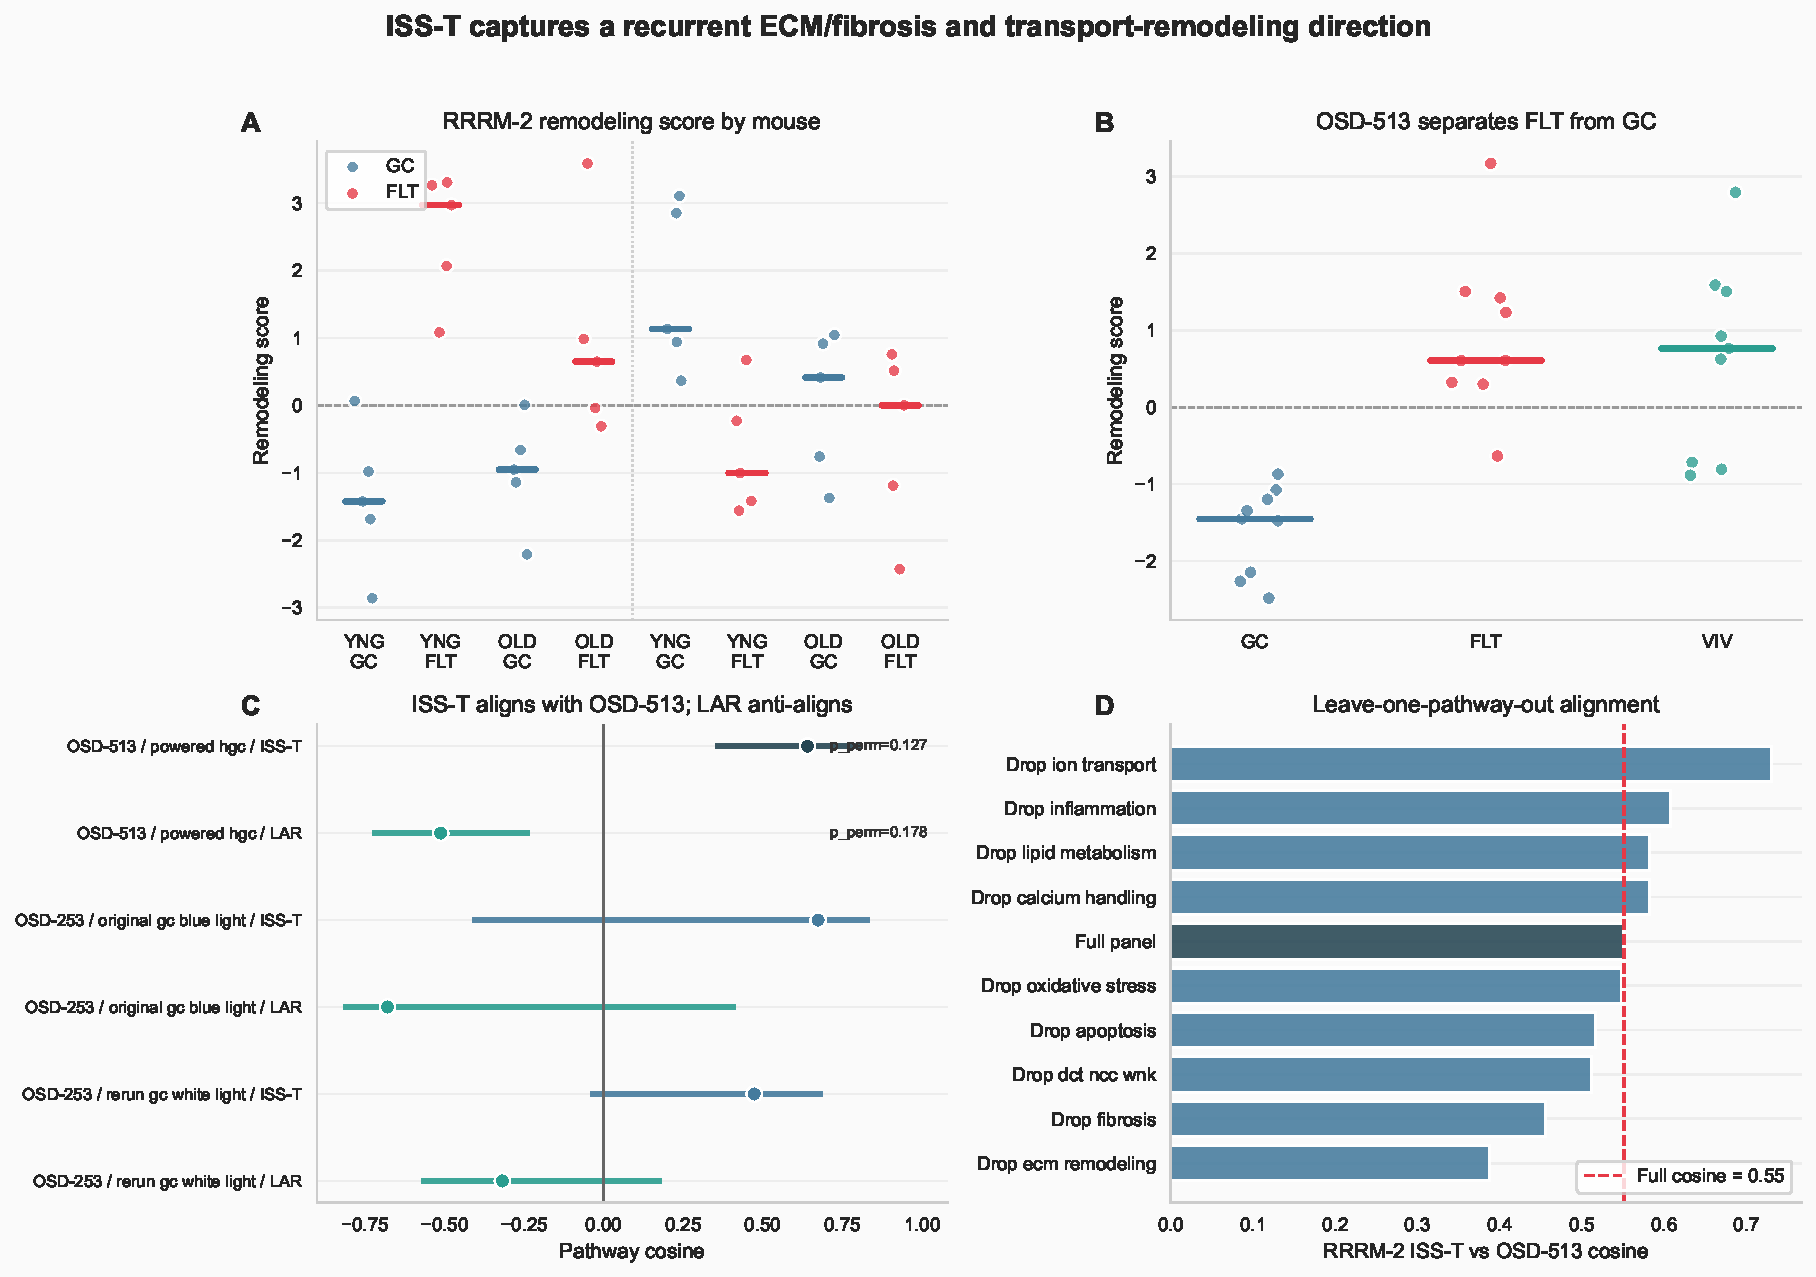
\includegraphics[width=\textwidth]{fig1_main_result_multipanel.pdf}
\caption{\textbf{Cross-cohort RNA recurrence.} RRRM-2 ISS terminal flight and OSD-513 show a recurring matrix-high / DCT-low RNA response. OSD-513 recurrence uses nine shared pathway features; the matched OSD-462 RNA anchor uses the 11-pathway multi-omic panel. Terminal-flight RNA remodeling recurs across cohorts, while live animal return is treated as recovery context.}
\label{fig:rnarecurrence}
\end{figure}

\begin{figure}[H]
\centering
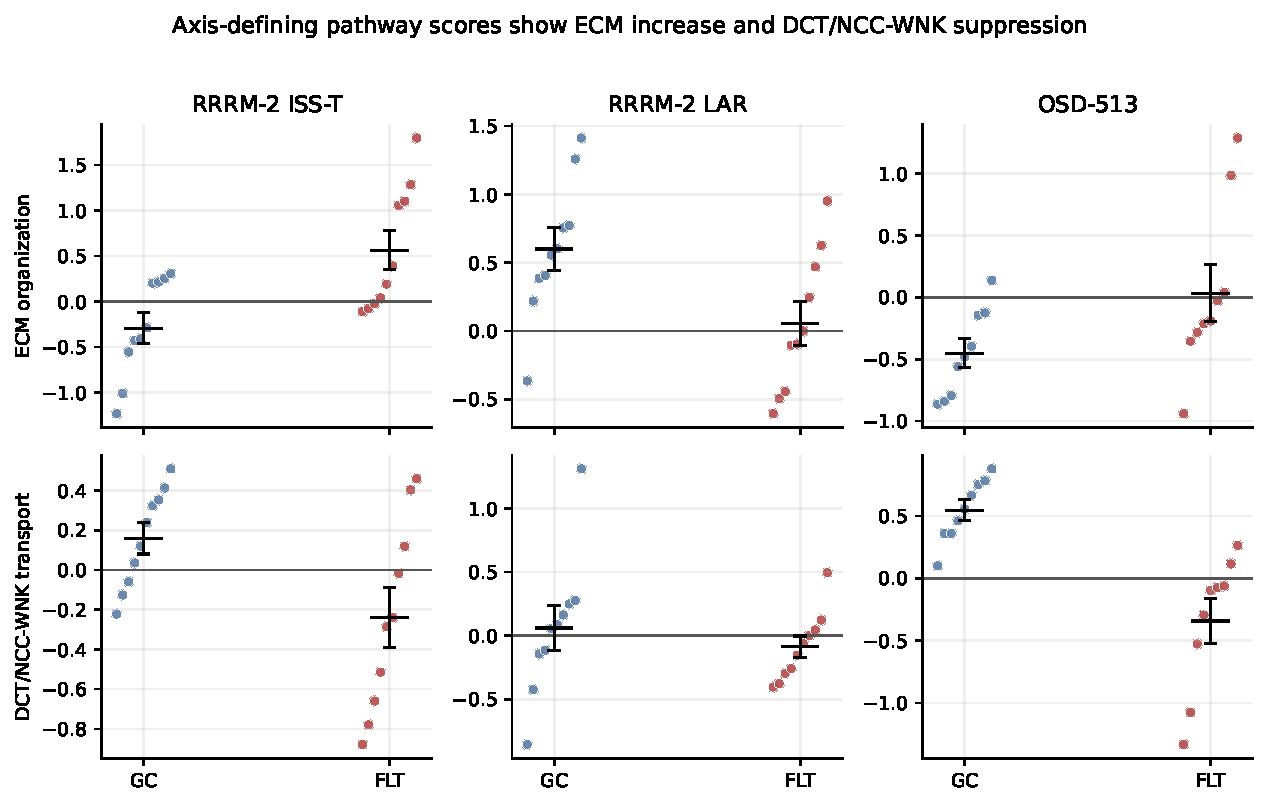
\includegraphics[width=\textwidth]{fig2_pathway_scores_by_flight.pdf}
\caption{\textbf{Axis-defining RNA pathway scores by flight.} Within-study standardized ECM/remodeling and DCT/NCC-WNK transport scores for RRRM-2 ISS terminal, RRRM-2 live animal return, and OSD-513. Points are individual animals; black summaries are group-level means with uncertainty. Flight raises ECM/remodeling and lowers DCT/NCC-WNK transport in the terminal-flight arms, the per-animal basis for the cross-cohort recurrence and the ECM-DCT differential.}
\label{fig:pathwayscoresmethods}
\end{figure}

\subsection{OSD-462 shows RNA-protein mismatch}

In OSD-462, the recurrent RNA pattern was not recapitulated as a protein-abundance signature. Targeted protein-abundance concordance---whether a gene set's RNA and protein flight effects agree in direction and magnitude---was null for every tested gene set. Matrix/ECM proteins moved opposite their transcripts (mean protein effect $-0.107$, $p=0.012$ against an abundance- and peptide-count-matched gene-set null; RNA--protein concordance $-0.40$), and the DCT/NCC-WNK protein set showed no clear abundance effect (mean $-0.044$). Total NCC protein abundance was essentially unchanged in flight ($+0.089$ log$_2$ units), serving as the total-abundance control for the phosphosite results below.

At genome scale, RNA and protein flight effects were decoupled rather than inverted (Spearman $-0.034$). This is the loose coupling expected of bulk tissue: transcript and protein abundance correlate only modestly even in matched, unperturbed tissue \citep{liu2016dependency}, and under a compositional shift---expanding interstitial and endothelial compartments diluting per-cell signals---bulk RNA tracks which cell types are present as much as how each cell regulates its proteins \citep{nido2020composition,avilacobos2020deconv}. Against that baseline the informative result is pathway-specific: of the curated panel, the one set with a protein effect testable against a matched null, matrix/ECM, was inverted (mean protein $-0.107$, RNA--protein concordance $-0.40$), its strong RNA induction reversed at protein, while the remaining sets were small and non-propagating (Table~\ref{tab:crosslayer}, Fig.~\ref{fig:crosslayer}). The consequence is concrete: a reader with only the RNA data would infer that matrix-remodeling proteins accumulate in the spaceflight kidney, which the protein layer does not show. The recurrent RNA signature is thus a tissue-context readout, not a protein-output program, and is insufficient on its own for protein-level inference; the matched protein and phosphorylation layers recover the transporter-regulatory deficit.

% Table tab:crosslayer relocated to Supplementary Information (see appendix).

\begin{figure}[H]
\centering
\includegraphics[width=0.9\textwidth]{v11_cross_layer_heatmap.pdf}
\caption{\textbf{Cross-layer direction by pathway in OSD-462.} Each cell shows the within-layer flight effect (color, $z$) and its direction ($\uparrow$ up, $\downarrow$ down, $\approx$ flat) for the RNA, protein, and phosphosite layers across the 11 curated pathways, ordered by RNA effect. Remodeling sets are induced at RNA but fall or stay flat at protein, and DCT/NCC-WNK transport falls at RNA and phosphorylation while its protein rises: no pathway shows strong, nontrivial RNA-to-protein propagation, so the bulk RNA response reads as tissue context rather than a protein-output program.}
\label{fig:crosslayer}
\end{figure}

Calibrating these direction calls against the matched null sharpened them into explicit layer assignments and recovered both pre-registered endpoints (Methods; \path{src/v11/rna_protein_propagation.py}). Matrix/ECM and TLR4/innate emerged as calibrated protein inversions, the protein layer moving opposite the RNA direction beyond the abundance- and peptide-count-matched null (matrix/ECM signed-mean protein $-0.107$, inverse-signed-mean BH $q=0.091$; TLR4/innate inverse-slope BH $q=0.078$). A further three pathways behaved as RNA-to-phospho carries, their RNA direction reappearing at the phosphosite parent mean rather than at protein abundance: DCT/NCC-WNK transport (31\% of RNA-directional members carried at phospho, $n=13$), broad tubular transport, and S1P/S1PR3. The pre-registered matrix/ECM inversion and DCT/NCC-WNK phospho-carry were thus both confirmed, and the three carry candidates extend the pattern beyond what was hypothesized (Fig.~\ref{fig:propagation}; Benjamini-Hochberg within the 11-pathway family).

\begin{figure}[t]
\centering
\includegraphics[width=\linewidth]{../data/results/run_20260606_v11_layer_specificity/figures/v11_rna_protein_propagation.pdf}
\caption{\textbf{Calibrated RNA$\to$protein propagation per pathway.} Left: pathway signed-mean protein effect (signed by the RNA pathway-mean direction) with the $95\%$ central interval of the abundance$\times$peptide-count matched null ($n=10{,}000$ draws); pathways whose interval falls below zero are calibrated protein-inverted. Right: per-gene class fraction stack for RNA-directional pathway members (RNA-to-protein concordant; RNA-to-phospho carried; RNA/protein inverted; RNA only/other). The matrix/ECM inversion and the DCT/NCC-WNK phospho-carry are the two pre-registered layer-assignment outcomes; both survive matched-null calibration.}
\label{fig:propagation}
\end{figure}

The transporter-regulatory deficit instead appeared at the phosphorylation layer. Because NCC is activated by WNK--SPAK/OSR1 phosphorylation of its N-terminal regulatory sites, this layer rather than total abundance reports transporter activation, so flat NCC protein with suppressed regulatory phosphosites indicates reduced activation despite preserved abundance. NCC N-terminal phosphosite features fell by approximately 0.79--0.99 log$_2$ units, and the composite p65;p68 feature fell by $-1.563$ ($p=9.3\times10^{-7}$). SPAK position features p366 and p383 were also suppressed. Non-regulatory NCC sites were comparatively flat. These suppressed N-terminal and SPAK sites are concordant with the antibody-validated NCC dephosphorylation reported by Cosmic Kidney Disease \citep{siew2024cosmic}. In OSD-462, the NCC/SPAK/WNK phosphorylation pattern occurs without a corresponding decrease in total NCC protein abundance or broad RNA-to-protein propagation of the flight RNA program. Targeted KSEA over curated substrates was directionally consistent with reduced SPAK/OSR1 and WNK axis output and is read as pathway coherence (Methods).

The strongest independent corroboration came from the unbiased kinome-wide screen. Scoring all quantified Ser/Thr phosphosites against the Johnson et al.\ kinase atlas \citep{johnson2023atlas}, without the curated substrate list, recovered \gene{WNK1} and \gene{WNK3} among the most suppressed kinase outputs in the kidney ($z=-4.87$, $q=5.4\times10^{-6}$, 101 atlas substrates; and $z=-4.69$, $q=1.3\times10^{-5}$, 208 substrates). An orthogonal method sharing no inputs with the targeted analysis thus reaches the same WNK axis, extending the result rather than restating it. The screen did not recover the SPAK/OSR1 arm---SPAK/STK39 (atlas label STLK3) and OSR1 outputs were slightly positive and \gene{WNK4} only nominally suppressed ($q=0.11$)---so SPAK/OSR1 suppression rests on the targeted curated substrates while the WNK component is independently confirmed.

Set against the five-cohort recurrence meta-analysis, the matched phosphoproteomic layer is where the transporter-regulatory deficit is clearest: the recurrent RNA signal is carried mainly by the matrix/ECM-high set (Stouffer $z=3.39$), whereas the DCT/NCC-WNK transport decrease is heterogeneous across cohorts ($z=-1.32$) and resolves into a defined effect only at the OSD-462 phosphosites.

\begin{table}[H]
\centering\small
\caption{\textbf{Selected OSD-462 WNK--SPAK/OSR1--NCC phospho-axis flight effects.} Space Flight minus Ground Control, log$_2$ scale.}
\label{tab:phospho}
\begin{tabular}{llrrl}
\toprule
Feature & Site & Flight effect & $p$ value & Role \\
\midrule
NCC (\gene{Slc12a3}) protein & --- & $+0.089$ & --- & total abundance control \\
NCC phospho & p53 & $-0.851$ & $3.8\times10^{-4}$ & N-terminal regulatory-position feature \\
NCC phospho & p65 & $-0.790$ & $3.5\times10^{-6}$ & N-terminal regulatory-position feature \\
NCC phospho & p68 & $-0.794$ & $3.3\times10^{-4}$ & N-terminal regulatory-position feature \\
NCC phospho & p89 & $-0.930$ & $6.6\times10^{-5}$ & additional N-terminal phosphosite \\
NCC phospho & p65;p68 & $-1.563$ & $9.3\times10^{-7}$ & composite position feature \\
NCC phospho & p96 & $+0.048$ & $0.48$ & non-regulatory control \\
NCC phospho & p120 & $+0.027$ & $0.78$ & non-regulatory control \\
SPAK (\gene{Stk39}) phospho & p366 & $-0.520$ & $1.7\times10^{-5}$ & kinase arm \\
SPAK (\gene{Stk39}) phospho & p383 & $-0.793$ & $2.8\times10^{-4}$ & kinase arm \\
\bottomrule
\end{tabular}
\end{table}

Position-only labels are used because the OSD-462 phosphosite table stores site positions, and residue-letter assignment depends on accession/isoform mapping. The p89 NCC feature is therefore reported as an additional N-terminal phosphosite rather than folded into the curated SPAK/OSR1 regulatory-position set without a separate residue-mapping citation.

\begin{figure}[H]
\centering
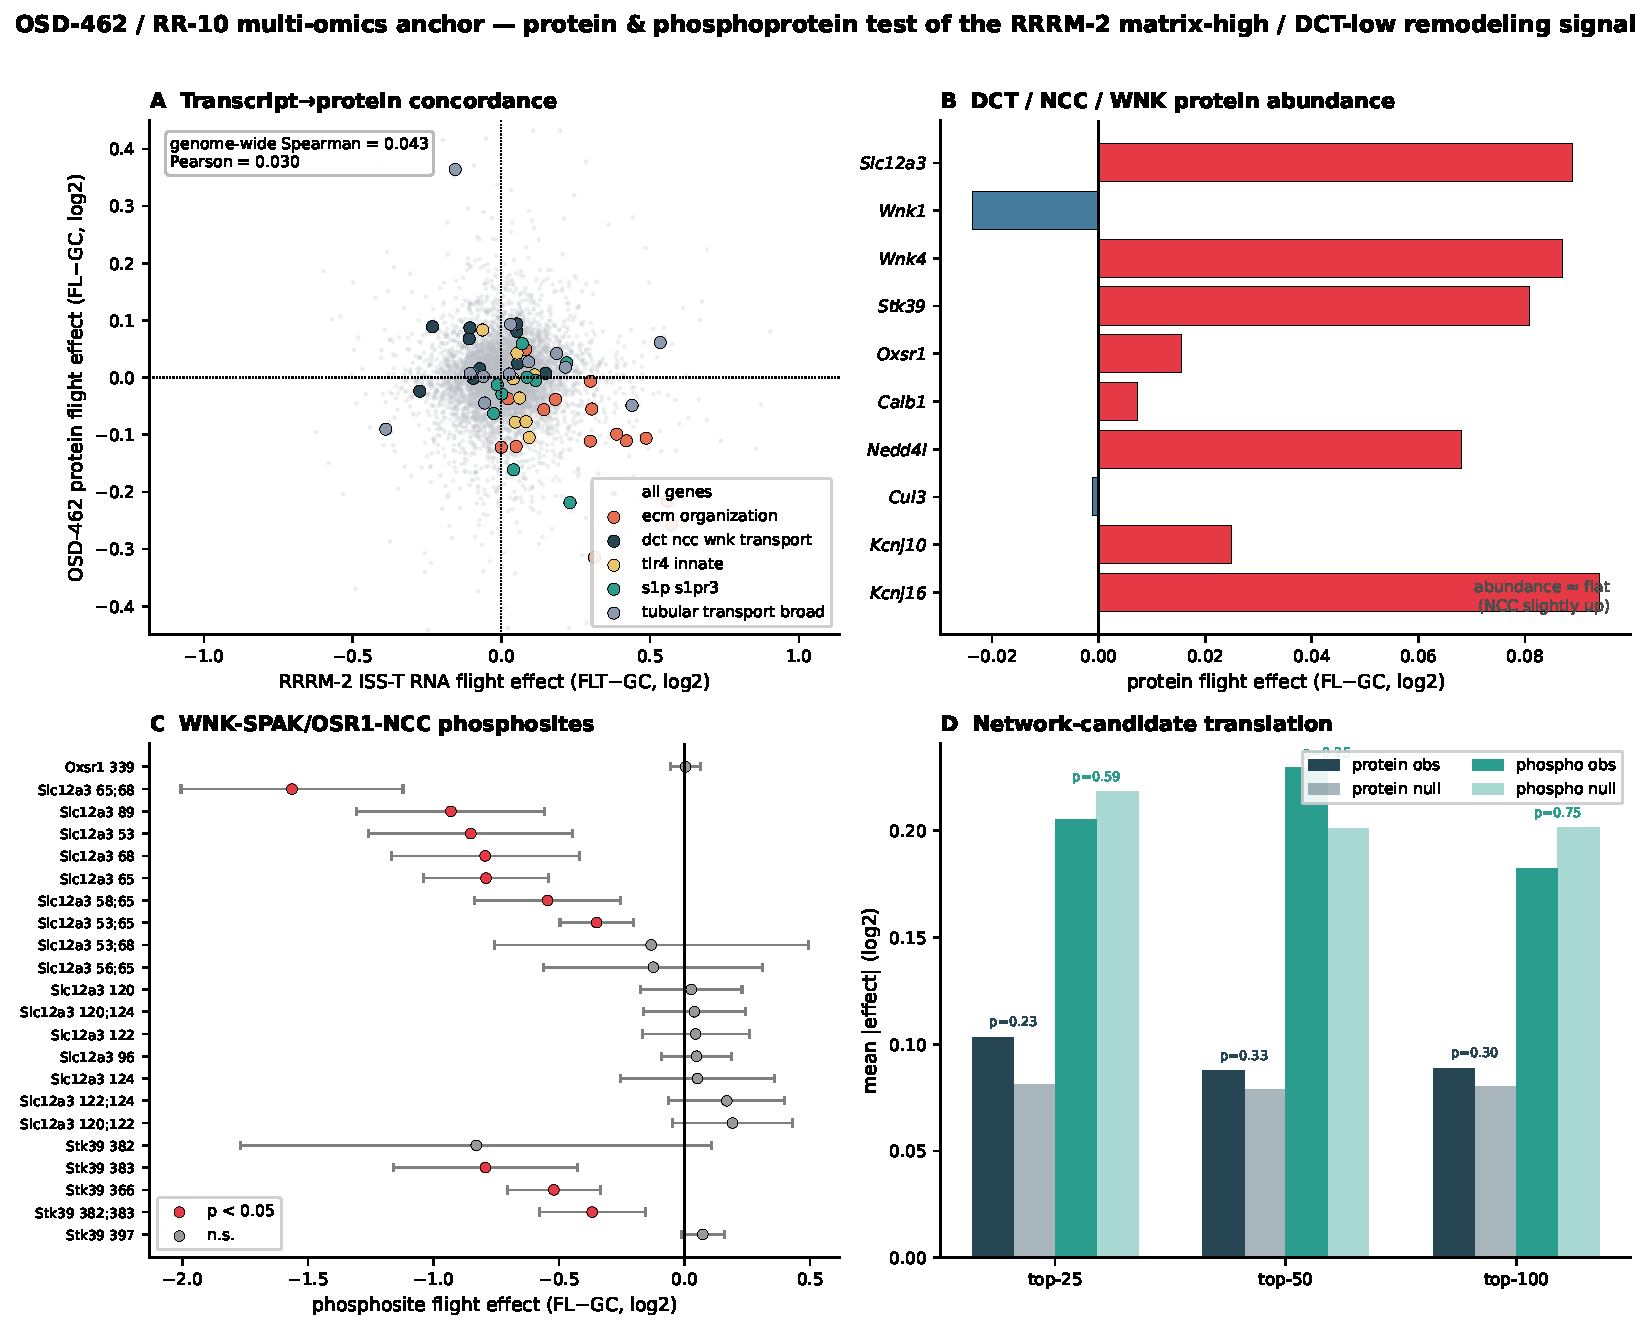
\includegraphics[width=\textwidth]{fig_osd462_multiomics_dashboard.pdf}
\caption{\textbf{OSD-462 RNA-protein mismatch.} Panel A is the matched OSD-462 RNA-versus-OSD-462-protein scatter (genome-wide Spearman $-0.034$): the recurrent RNA response is not matched by concordant protein-abundance changes. Panel B shows DCT/NCC-WNK protein abundance flat-to-slightly-positive, and Panel C shows the NCC/SPAK/WNK regulatory phosphosite cluster suppressed with total NCC protein flat, with phosphosites grouped into regulatory (NCC N-terminal, SPAK/OSR1) and non-regulatory sets.}
\label{fig:osd462}
\end{figure}

\begin{figure}[H]
\centering
\includegraphics[width=\textwidth]{v11_extension_kinome_recurrence.pdf}
\caption{\textbf{Kinome-wide and cross-cohort recurrence extensions.} The kinome-wide substrate-atlas KSEA independently recovers suppressed WNK1 ($q=5.4\times10^{-6}$) and WNK3 ($q=1.3\times10^{-5}$) output in OSD-462, whereas WNK4 ($q=0.11$) and the SPAK/OSR1 arm (OSR1 $z=+1.57$, n.s.) are not suppressed in the unbiased atlas; the five-cohort RNA recurrence meta-analysis shows stronger recurrence for the matrix/ECM-high remodeling set than for the DCT/NCC-WNK transport set. These analyses place the measured NCC/SPAK/WNK phosphosite endpoint in a broader WNK-output and remodeling context.}
\label{fig:kinomerecurrence}
\end{figure}

\subsection{The bulk DCT-low signal is partly explained by endothelial and stromal expansion}

Part of the bulk DCT-low signal reflects compartment shift rather than DCT-cell-intrinsic suppression. Across cohorts, DCT identity and DCT transport markers fell together while endothelial and stromal/fibroblast scores rose; as interstitial and endothelial cells expand they capture a larger share of the sequenced transcripts, lowering apparent DCT-gene levels even when surviving DCT cells transcribe normally. Within OSD-462, endothelial score increased in flight ($+1.00$, $p=0.036$) and stromal score increased directionally ($+0.67$, $p=0.054$). The endothelial score anti-correlated strongly with NCC regulatory phosphorylation across animals ($\rho=-0.762$, $p=0.0004$; Fig.~\ref{fig:endoscatter})---the strongest animal-level relationship in the dataset, which we decompose below---while DCT identity correlated positively with NCC regulatory phosphorylation ($\rho=+0.52$, $p=0.020$).

\begin{figure}[H]
\centering
\includegraphics[width=0.62\textwidth]{v11_endothelial_ncc_scatter.pdf}
\caption{\textbf{Per-animal endothelial score versus NCC regulatory phosphorylation in OSD-462} ($n=20$). Flight animals (red) carry higher endothelial/remodeling RNA scores and lower NCC regulatory phosphorylation, ground controls (blue) the reverse (Spearman $\rho=-0.762$, $p=0.0004$). This is the strongest animal-level relationship in the dataset and motivates the covariance decomposition below; as a bulk-tissue correlation it points to spatial and time-course testing rather than fixing causal or cell-resolved order. The relationship is carried by the flight/control contrast and, within condition, by the ground-control animals (ground control $\rho=-0.73$, flight $\rho=-0.20$), consistent with restricted range at $n=10$ per group.}
\label{fig:endoscatter}
\end{figure}

Animal-matched RNA and phosphoprotein scores moved together at group level: flight lowered the DCT transport RNA score ($-0.324$) and NCC regulatory phosphorylation score ($-1.298$). The condition-adjusted per-animal correlation was positive but not significant ($\rho=+0.365$, $p=0.113$), consistent with limited power at $n=20$. Non-regulatory NCC sites also correlated per animal with the DCT transport RNA score, so per-animal regulatory-site specificity is not claimed. The data therefore support group-level agreement against an interstitial/endothelial remodeling background. That this suppression is a real signal rather than a low-coverage artifact is reinforced by where the affected sites sit in the phosphoproteome: the suppressed NCC/SPAK regulatory phosphosites (\gene{Slc12a3} S53/S65/S68, \gene{Stk39} S382/S383) occupy the $99.1$--$99.4$ percentile of phosphoproteome effect magnitude, whereas the four non-regulatory NCC control sites (\gene{Slc12a3} S96/S120/S122/S124) sit at the $14.7$--$27.6$ percentile (companion results compendium); the suppression lives in the most-confidently-measured part of the phosphoproteome, not in a low-coverage tail.

\begin{table}[H]
\centering\small
\caption{\textbf{Animal-matched comparison of DCT transport RNA and NCC phosphorylation in OSD-462.}}
\label{tab:matched}
\resizebox{\textwidth}{!}{%
\begin{tabular}{lrrrrrr}
\toprule
Comparison & $n$ & RNA FLT$-$GC & phospho FLT$-$GC & Spearman all & $p$ & condition-adjusted Spearman \\
\midrule
Regulatory sites vs RNA & 20 & $-0.324$ & $-1.298$ & $+0.328$ & 0.158 & $+0.365$ \\
Regulatory + p89 sensitivity & 20 & $-0.324$ & $-1.299$ & $+0.343$ & 0.139 & $+0.325$ \\
Non-regulatory sites vs RNA & 20 & $-0.324$ & $-0.299$ & $+0.555$ & 0.011 & $+0.474$ \\
Regulatory vs RNA, \gene{Slc12a3} removed & 20 & $-0.247$ & $-1.298$ & $+0.301$ & 0.198 & $+0.364$ \\
\bottomrule
\end{tabular}
}
\end{table}

\subsection{Flight-suppressed phosphosites are enriched in distal-nephron subtype-prior extremes}

Flight-suppressed phosphosites are not a random sample of the kidney phosphoproteome: they concentrate in the parent genes that define distal-nephron identity, and---unexpectedly---the signal that survives the most stringent observability-matched permutation is the DCT2-leaning extreme, not the canonical DCT1 anchors. The sensitivity ladder establishing this follows.

The phosphosite-prior analysis evaluated whether flight-suppressed OSD-462 whole-kidney phosphosites were concentrated in parent genes with distal-nephron subtype-prior expression. Phosphosites were mapped to parent genes and then to an external DCT1/DCT2 transcriptomic prior, so the analysis tests parent-gene prioritization in whole-kidney phosphoproteomics.

GSE228367 provided a native DCT1/DCT2 transcriptomic prior. Marker checks supported the expected subtype structure: \gene{Slc12a3} was present in both subtypes but higher in DCT1, \gene{Pvalb} and \gene{Trpm6} were DCT1-high, \gene{Stk39} and \gene{Wnk4} were DCT1-leaning, and \gene{Trpv5}/\gene{Calb1} were DCT2-high. Because strict binary marker sets were sparse, the analysis used continuous DCT1 enrichment scores, DCT1-top percentile bins, and DCT2-leaning low-DCT1-score percentile bins. The DCT2-leaning bin is defined by the lowest DCT1 enrichment scores rather than by positive DCT2 specificity; it captures bona fide DCT2/CNT markers (\gene{Trpv5}, \gene{Calb1}; Table~\ref{tab:dct2validation}) at its expected end but can also include broadly expressed or low-DCT1 genes, so we label it ``DCT2-leaning'' rather than DCT2-specific. Leave-one-replicate-out mean-difference priors were stable (Jaccard 0.85--0.86 against the primary DCT1-top-decile parent-gene bin), while log-ratio and rank-average scores changed bin membership more strongly.

Flight-suppressed OSD-462 whole-kidney phosphosites were enriched in DCT-subtype-prior extremes. At the phosphosite-row level (each quantified phosphosite counted once, so a multiply-phosphorylated gene contributes several rows), the DCT1 top-decile bin was the strongest primary result (OR 1.51, q=$1.33\times10^{-11}$), and it remained enriched after anchor-gene exclusion, NCC-site exclusion, exclusion of composite/multi-position rows (OR 1.38, q=$2.0\times10^{-6}$), one phosphosite row per parent gene (OR 1.49, q=$6.59\times10^{-4}$), and the stricter single-position-row-per-parent-gene reduction (OR 1.48, q=$9.05\times10^{-4}$). Parent-gene Fisher testing was also supportive (OR 1.52, q=$1.90\times10^{-4}$), and parent-gene cluster bootstrap intervals remained above one (95\% CI 1.22--1.81). The signal weakened in the covariate-adjusted parent-gene logistic model (OR 1.14, q=0.424) and attenuated under the observability-matched parent-gene permutation preserving site count, peptide count, parent abundance, and missingness (empirical $p=0.107$). DCT1 enrichment is thus strong at the row and parent-gene level but conditional on observability structure---a pattern the DCT2-leaning bin does not share.

The DCT2-leaning bin is the one that strengthens where DCT1 attenuates. Defined as the lowest-DCT1-score decile, it was enriched at the row level (OR 1.29, q=$1.30\times10^{-5}$), after composite-site exclusion (OR 1.33, q=$1.30\times10^{-5}$), in the one-row-per-parent-gene reduction (OR 1.68, q=$4.62\times10^{-6}$), in the stricter single-position reduction (OR 1.52, q=$2.91\times10^{-4}$), at parent-gene level (OR 1.82, q=$3.29\times10^{-8}$), and---decisively---under the same matched parent-gene permutation that DCT1 fails (empirical $p=0.017$). Joint logistic models including both decile flags attenuated each nominal endpoint (DCT1 OR 1.17, q=0.320; DCT2 OR 1.27, q=0.104), so the supported claim is enrichment across the distal-nephron subtype prior rather than exclusivity at either pole. The DCT1 top decile remains biologically motivated because NCC, SPAK, and WNK4 are DCT1-leaning by the GSE228367 mean-difference prior. The DCT2/CNT transition also carries the aldosterone-sensitive distal segment and the principal calcium-handling machinery (\gene{Trpv5}, \gene{Calb1}) together with electrogenic sodium and potassium transport, whereas magnesium handling (\gene{Trpm6}) is DCT1-leaning; this makes the DCT2-leaning bin biologically plausible in a broad distal-transport phenotype. Table~\ref{tab:dct2compare} and Fig.~\ref{fig:dctladder} summarize the DCT1/DCT2 evidence ladder. Spaceflight therefore acts selectively on the regulatory phosphorylation of the distal-transport program rather than diffusely across kidney signaling, which is what lets a whole-kidney phosphoproteome speak to a specific nephron segment.

\begin{table}[H]
\centering\small
\caption{\textbf{DCT1-high versus DCT2-leaning extreme-bin enrichments.} The DCT2-leaning bin contains the 10\% of detected parent genes with the lowest DCT1 enrichment score. Both extremes are tested with the same one-sided Fisher exact alternative. In several parent-gene-aware sensitivities the DCT2-leaning odds ratio is the larger of the two, and the DCT2-leaning bin survives the matched parent-gene permutation (final row).}
\label{tab:dct2compare}
\resizebox{\textwidth}{!}{%
\begin{tabular}{lrrrrl}
\toprule
Analysis & DCT1 OR & DCT1 q & DCT2 OR & DCT2 q & Read \\
\midrule
Row primary $p<0.05$ & 1.51 & $1.33\times10^{-11}$ & 1.29 & $1.30\times10^{-5}$ & DCT1 stronger \\
Composite rows excluded & 1.38 & $2.0\times10^{-6}$ & 1.33 & $1.30\times10^{-5}$ & similar \\
One row per parent gene & 1.49 & $6.59\times10^{-4}$ & \textbf{1.68} & $\mathbf{4.62\times10^{-6}}$ & DCT2 larger \\
Single-position row per gene & 1.48 & $9.05\times10^{-4}$ & \textbf{1.52} & $\mathbf{2.91\times10^{-4}}$ & both pass \\
Parent-gene Fisher & 1.52 & $1.90\times10^{-4}$ & \textbf{1.82} & $\mathbf{3.29\times10^{-8}}$ & DCT2 larger \\
Matched parent-gene permutation & 1.51 & 0.107 & \textbf{1.70} & \textbf{0.017} & DCT1 attenuates \\
\bottomrule
\end{tabular}
}
\end{table}

\begin{figure}[H]
\centering
\includegraphics[width=\textwidth]{v11_dct1_vs_dct2_evidence_ladder.pdf}
\caption{\textbf{DCT1-high versus DCT2-leaning enrichment evidence ladder.} \emph{DCT1-high enrichment is strongest at the phosphosite-row level but does not survive the observability-matched parent-gene permutation, whereas the DCT2-leaning bin is stronger in several parent-gene-aware tests and survives it; the supported claim is distal-nephron subtype-prior enrichment, not DCT1-exclusive localization.} Odds ratios are shown across row-level, parent-gene-aware, adjusted, bootstrap, and matched-permutation summaries.}
\label{fig:dctladder}
\end{figure}

% Table tab:dct1counts relocated to Supplementary Information (see appendix).

\subsection{Subtype-prior enrichment survives abundance and composition adjustment}

Parent-protein and compartment-score adjustment retained the DCT1 top-decile enrichment. In the full parent-protein plus DCT/endothelial/stromal model, top-decile enrichment remained significant (OR 1.30, q=0.00158). A composition-PC sensitivity was similar (OR 1.38, q=$6.53\times10^{-5}$). The top-quartile result attenuated in the full model (OR 1.05, q=0.282), indicating that the DCT1 component is concentrated in the top-decile subset. The same robustness holds against proteome detectability: substituting a per-channel-missingness-extended matched null for the standard abundance$\times$peptide-count null does not shift any per-pathway slope BH $q$-value by more than $0.041$ (matrix/ECM $0.889\to0.870$; DCT/NCC-WNK $0.910\to0.870$; companion results compendium), so the cross-layer pattern is not an artifact of which proteins are easiest to quantify.

The adjusted models redefine the suppressed set on each residual scale: the raw M0 model contained 2,430 nominally suppressed single-position sites, while the full M4 model contained 1,390. A fixed-set sensitivity therefore tracked the M0 suppressed sites across adjustment rather than redefining membership. In the M4 full model, 99.3\% of M0 suppressed sites with matched covariates remained negative (mean adjusted effect $-0.295$), and the DCT1 top-decile subset showed the same pattern (99.7\% negative; mean adjusted effect $-0.303$). Covariate diagnostics showed nontrivial sample-level collinearity in $n=20$ animals (endothelial--stromal correlation $r=0.86$, stromal-score VIF 6.59), which inflates standard errors but does not change the direction of the result: the DCT1 top-decile odds ratio stayed above one and significant under each covariate added on its own (M1 parent-protein OR 1.55, M2 DCT-identity OR 1.36, M3 endothelial/stromal OR 1.24), so the retained signal is not an artifact of the collinear full-model specification.

Continuous DCT1-reference models did not support a broad gradient effect. The two-stage full model produced a positive, non-significant DCT1 coefficient, and the one-shot flight-by-DCT1 interaction was directionally negative but weak. The result is better described as subset enrichment than as a continuous DCT1-gradient model.

\begin{figure}[H]
\centering
\includegraphics[width=0.86\textwidth]{v11_parent_protein_composition_sensitivity.pdf}
\caption{\textbf{Parent-protein and bulk-composition sensitivity ladder.} Parent-protein and compartment-score adjustments retain the DCT1 top-decile signal across the M0--M5 ladder.}
\label{fig:composition}
\end{figure}

A final normalization sensitivity confirmed that the enrichment is not an artifact of the TMT channel-median shift. Raw flight phosphosite channels carried lower scaled intensities than ground-control channels in both plexes (mean per-channel $\log_2$ median ${\sim}0.13$ below ground control), whereas protein channels were stable (${\sim}0.01$). Primary per-site effects are estimated within plex after per-channel median centering; under that centered scale, the median site effect was $+0.007$ versus $-0.135$ on the uncentered scale. Re-running the DCT-prior enrichment on uncentered effects increased the suppressed-site fraction (15\% to 38\%) but retained subtype-prior enrichment (DCT1 top-decile OR 1.27, DCT2-leaning OR 1.17), while the centered primary estimates were stronger (OR 1.51 and 1.29; Fig.~\ref{fig:tmtqc}). The enrichment therefore follows relative phosphosite ranking after within-plex normalization, not the global channel-median shift (its interpretation as subtype-prior enrichment rather than an absolute dephosphorylation magnitude is taken up in Limitations).

\subsection{Exploratory covariance decomposition relates remodeling scores to NCC regulatory phosphorylation}

The endothelial score anti-correlated strongly with NCC regulatory phosphorylation across the OSD-462 flight and ground-control animals ($n=20$), motivating the covariance-decomposition summaries reported here. The implemented models used linear summaries with bootstrap or normal-approximation OLS uncertainty rather than a full SEM or \code{brms} fit. Endothelial and matrix/endothelial composite scores covaried negatively with NCC regulatory phosphorylation under the conditioning choices, while direct flight effects persisted. Stromal/fibroblast and DCT identity summaries were directionally consistent but less precise.

The per-animal OSD-462 data are compatible with a remodeling-linked transporter hypothesis and with parallel flight effects on remodeling and transporter phosphorylation; which of the two holds is taken up in the Discussion, since cross-sectional bulk data cannot order them.

\subsection{Public perturbation references refine robustness and future experiments}

The distal-nephron subtype-prior result and the matched multi-omic mismatch leave the upstream signal for WNK--SPAK--NCC phosphosite suppression unresolved. Three public references constrain it from different directions: a parent-protein normalization that tests robustness, a low-potassium DCT reference that tests directionality against a known physiological perturbation, and an injury/repair spatial atlas that turns the result into a testable prediction.

The subtype-prior enrichment is robust to parent-protein abundance. A paired animal-level phosphosite-minus-parent-protein model supported both the DCT1-high (OR 1.56, q=$1.90\times10^{-10}$) and DCT2-leaning (OR 1.54, q=$2.22\times10^{-10}$) deciles, and the simpler per-site parent-protein-normalized re-test held for the DCT1 top decile (OR 1.52, 95\% CI 1.36--1.70, q=$1.04\times10^{-11}$) across anchor-gene, NCC-site, and representative-row sensitivities. The transporter-regulatory signal is therefore not an artifact of parent-protein abundance.

Low extracellular potassium normally drives the DCT to phosphorylate and activate NCC through the WNK--SPAK pathway, raising distal sodium reabsorption to sustain potassium secretion; spaceflight moves these sites the opposite way, so a low-potassium DCT reference (GSE228367 KD vs NK pseudobulk) is a natural directional test. In the 14-gene DCT/WNK transport-target subset, all three spaceflight cohorts moved opposite the low-K activation response (OSD-462 RNA cosine $-0.286$, 95\% CI $-0.752$ to $0.458$, Spearman $\rho=-0.420$, $p=0.135$, q=0.218; RRRM-2 ISS terminal $-0.311$; OSD-513 $-0.146$), and 10 of the 14 genes---including \gene{Slc12a3}, \gene{Wnk1}, \gene{Klhl3}, \gene{Cul3}---flipped in OSD-462, while genome-wide cosines were near zero, so the anti-alignment is concentrated in transport targets rather than spread across the transcriptome. The result stayed below the pre-specified promotion threshold (cosine $<-0.3$ with a confidence interval excluding zero), so it is retained as a focused transport-target hypothesis rather than a primary mechanistic claim.

An external ischemia-reperfusion spatial atlas converts the result into a spatial prediction. In GSE269622 Visium, the 10-gene DCT-transport score fell in DCT-adjacent spots at day 14 (mean difference $-0.044$) and week 6 ($-0.034$) while DCT-marker-high spots themselves rose, suggesting that in spaceflight kidney the DCT/NCC-WNK loss may concentrate in DCT-adjacent remodeling neighborhoods rather than in the DCT core---a hypothesis a spaceflight spatial experiment can test directly. Spot-level p values and full niche counts are in the compendium.

Two references that might have named an upstream mechanism were coverage-limited, but informatively so. The PXD001729 dDAVP/mpkDCT phosphoproteome shared 60 single sites with OSD-462 but none of the 14 transport targets, and KLHL3/CUL3-mediated WNK turnover could not be probed (\gene{Klhl3} had zero quantified phosphosites, \gene{Cul3} one, and no public kidney ubiquitinomics exist). The informative result is the negative one: WNK, SPAK, and NCC protein abundances were flat to slightly positive, which argues against a degradation-driven loss of these proteins and points instead toward ionic/osmotic suppression of WNK--SPAK \emph{activity}---the same direction implied by the low-K reference.

Across these references the subtype-prior enrichment survives parent-protein normalization, the transport-target anti-alignment and the flat-abundance result both point toward activity-level rather than abundance-level regulation, and the spatial atlas supplies a concrete next experiment; the identity of the upstream WNK-suppressing signal remains the open question. The full perturbation-reference dashboard and branch tables are in the companion compendium.

\begin{figure}[H]
\centering
\includegraphics[width=\textwidth]{v11_perturbation_triangulation.pdf}
\caption{\textbf{Public perturbation-reference checks around the spaceflight DCT/phosphoproteomic signature.} (A) Low-potassium DCT response versus spaceflight RNA across gene subsets. (B) The focused 14-gene DCT/WNK transport-target directions across the low-K reference and three spaceflight cohorts. (C) External IRI Visium DCT-transport across the repair time course in DCT-marker-high versus DCT-adjacent spots. These panels are external-reference context and spatial predictions, not spaceflight spatial validation; parent-protein-normalized robustness is reported in the text.}
\label{fig:perturbation}
\end{figure}

\subsection{Network, cross-species, and translational constraints}

Cross-species and translational analyses placed two further constraints on the model. The first is a methodological integrity check: the genes prioritized by the LIONESS/node2vec network analysis did not enrich among OSD-462 protein- or phosphoprotein-changing genes. This is a deliberately strong negative---it shows that the phosphoproteomic signal is not merely recovering network-hub genes, and that the network method did not manufacture the result by routing through highly connected nodes. Three further comparisons were factual checks: live-return vectors attenuated or anti-aligned rather than reversing cleanly; OSD-253 showed TLR4/innate association without strict TLR4 requirement; and projection onto an aging reference showed no accelerated-aging alignment (their interpretation as boundary conditions is taken up in the Discussion).

The second constraint is translational. In the NASA Twins flight subject, urine and clinical-chemistry directions collapsed onto three physiological axes---aldosterone/fluid handling, water balance, and DCT transport---all directionally aligned with the mouse-derived predictions. The human urine axis is therefore directionally concordant but underpowered: a single flight trajectory whose by-axis sign test is not significant ($p=0.25$) and whose \gene{AQP2} direction was read from a published figure. Quantitative validation would require machine-readable inflight distal-nephron or urine-proteomic measurements across multiple subjects, which the post-flight OSD-656 urine-inflammation context does not yet provide. The LINCS/CMap screen (50 up / 50 down query, 473,647 scored Level-5 signatures after \code{sig\_info} merge) is retained for perturbagen-class hypothesis generation rather than as model support. Detailed tables are in the companion compendium.

% =====================================================================
\section{Discussion}

\begin{figure}[t]
\centering
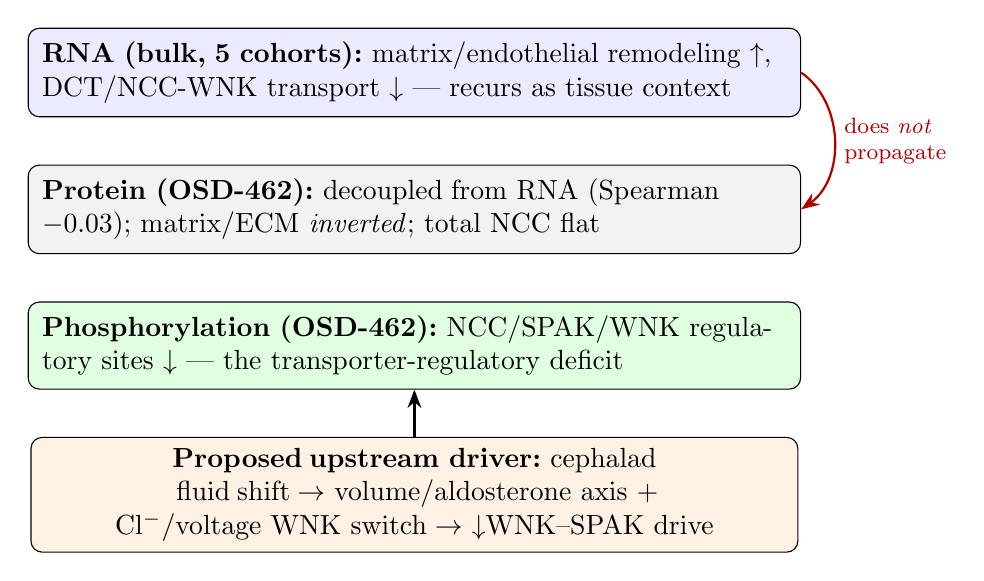
\begin{tikzpicture}[>=Stealth, node distance=6mm,
  layer/.style={draw, rounded corners, align=left, text width=0.78\textwidth, minimum height=11mm, inner sep=5pt},
  drv/.style={draw, rounded corners, align=center, fill=orange!10, text width=0.78\textwidth, inner sep=4pt}]
\node[layer, fill=blue!8] (rna) {\textbf{RNA (bulk, 5 cohorts):} matrix/endothelial remodeling $\uparrow$, DCT/NCC-WNK transport $\downarrow$ --- recurs as tissue context};
\node[layer, fill=gray!10, below=of rna] (prot) {\textbf{Protein (OSD-462):} decoupled from RNA (Spearman $-0.03$); matrix/ECM \emph{inverted}; total NCC flat};
\node[layer, fill=green!12, below=of prot] (phos) {\textbf{Phosphorylation (OSD-462):} NCC/SPAK/WNK regulatory sites $\downarrow$ --- the transporter-regulatory deficit};
\node[drv, below=of phos] (drv) {\textbf{Proposed upstream driver:} cephalad fluid shift $\rightarrow$ volume/aldosterone axis $+$ Cl$^-$/voltage WNK switch $\rightarrow$ $\downarrow$WNK--SPAK drive};
\draw[->, red!70!black, thick] (rna.east) to[bend left=55] node[right, font=\footnotesize, align=left]{does \emph{not}\\propagate} (prot.east);
\draw[->, thick] (drv) -- (phos);
\end{tikzpicture}
\caption{\textbf{Model: the spaceflight kidney response is layer-resolved.} The recurrent bulk-RNA remodeling state does not propagate to protein abundance (the matrix/ECM set is inverted at protein), so the RNA layer is a tissue-context readout. The transporter-regulatory deficit is carried by NCC/SPAK/WNK regulatory phosphorylation, which we propose is driven by reduced WNK--SPAK activity downstream of the microgravity fluid shift---through the volume/aldosterone axis, the chloride/voltage potassium switch, or both. The driver arrow is a hypothesis; the layer pattern is the result.}
\label{fig:model}
\end{figure}

\subsection{Main interpretation}

The central result is that the spaceflight kidney transporter phenotype is a regulatory-phosphorylation event reaching across the distal nephron, and that the bulk transcriptome does not report it. Across mouse kidney spaceflight cohorts the dominant recurring RNA component was matrix/endothelial remodeling, with weaker DCT/NCC-WNK transport suppression (Fig.~\ref{fig:model}); in OSD-462/RR-10 multi-omics that RNA state did not behave as a protein-abundance program (RNA and protein decoupled at genome scale, Spearman $-0.034$; targeted protein concordance null; the one null-tested set, matrix/ECM, inverted; DCT/NCC-WNK protein flat-to-positive while RNA fell). The transporter-regulatory signal was sharpest at the phosphorylation layer.

Reduced NCC regulatory phosphorylation against flat total abundance indicates reduced NCC activation and lower distal sodium-chloride reabsorption; through the well-characterized coupling of the distal nephron, this extends to potassium, calcium, and magnesium handling. The molecular chain from regulatory phosphorylation to distal electrolyte balance is therefore supported.

Cosmic Kidney Disease established spaceflight-associated NCC/distal-nephron dephosphorylation in RR-10/OSD-462 \citep{siew2024cosmic}; on the same animals, the present analysis adds what that endpoint alone could not show. The RNA, protein, and phosphoprotein layers \emph{disagree}: the recurrent matrix/endothelial RNA state fails to reach protein abundance while the transporter signal concentrates in regulatory phosphorylation, which we then rank against a DCT1/DCT2 subtype prior. The divergence is the informative part---the RNA and protein layers systematically diverge while phosphorylation aligns with the established endpoint, and an unbiased kinome-wide screen independently corroborates the WNK arm. The transporter-regulatory deficit is thus a phosphorylation-layer event embedded in tissue remodeling, not a transcriptional or abundance program, and phosphorylation is the layer future spaceflight kidney studies should measure directly.

\subsection{The distal-nephron subtype-prior signal and the upstream mechanism}

Flight-suppressed phosphosites concentrate in the parent genes that define distal-nephron identity, and that concentration is strongest, and most permutation-robust, at the DCT2-leaning end. Because OSD-462 is whole-kidney phosphoproteomics and GSE228367 an external transcriptomic reference, their intersection prioritizes parent genes rather than assigning a cell of origin; within that frame the suppressed phosphosites are overrepresented at distal-nephron subtype-prior extremes, across both DCT1-high and DCT2-leaning bins.

The DCT1 top decile stays biologically anchored: \gene{Slc12a3}, \gene{Stk39}, and \gene{Wnk4} fall in it under the primary mean-difference score, and leave-one-replicate-out DCT1-top and DCT2-leaning bins are stable for that score (Jaccard $\approx0.85$--$0.86$). Parent-gene Fisher, cluster bootstrap, matched permutation, threshold-free, and parent-protein/composition-aware analyses reduce the simplest row-amplification and abundance explanations, while the parent-gene logistic and matched-permutation results hold the interpretation at parent-gene enrichment rather than DCT1 exclusivity or cellular localization. The DCT1-high bin is strong at the row level but attenuates under the matched permutation ($p=0.107$) where the DCT2-leaning bin holds, so the supported claim is subtype-prior enrichment led by the DCT2-leaning extreme, with DCT1 anchored but more conditional.

The DCT2-leaning result is the more provocative half: the canonical NCC/SPAK/WNK anchors are DCT1-leaning, yet the DCT2-leaning bin is the one that survives observability-matched permutation. The bin's specific end contains canonical DCT2/CNT and aldosterone-sensitive markers (\gene{Trpv5}, \gene{Calb1}, \gene{Scnn1b/g}, \gene{Nedd4l}, \gene{Sgk1}; Table~\ref{tab:dct2validation}), but because it is defined by the lowest DCT1 score it also contains broadly expressed low-DCT1 genes; the DCT2/CNT-program reading below is therefore a biological hypothesis layered on a low-DCT1 statistical bin, not a cell-type assignment. One reading is that flight suppresses a phosphoregulatory program of the aldosterone-sensitive distal nephron that is broader than NCC itself. The DCT2/CNT transition is where the SGK1--NEDD4L axis tunes ENaC, where the calcium-transport machinery (\gene{Trpv5}, \gene{Calb1}) is regulated, and where WNK--SPAK signaling also acts on ROMK (\gene{Kcnj1}) and the K--Cl cotransporters \citep{subramanya2014dct,richardson2008wnk,arroyo2011aldosterone}; loss of regulatory phosphorylation on these DCT2/CNT-expressed substrates would register as DCT2-leaning enrichment without requiring NCC itself to be DCT2-specific. That would broaden the phenotype from sodium-chloride reabsorption alone toward coupled potassium and calcium handling in the aldosterone-sensitive segment---a hypothesis that DCT-subtype-resolved phosphoproteomics could test directly by asking which DCT2/CNT kinase substrates lose phosphorylation in flight.

A candidate upstream signal is now testable rather than simply open. A mineralocorticoid/aldosterone-axis score was directionally suppressed across cohorts (meta effect $-0.84$, $p=0.060$; strongest in OSD-513 and OSD-462) and tracked the NCC/WNK transport score almost perfectly across cohorts (Spearman $\approx1.0$; Fig.~\ref{fig:aldo}), consistent with reduced aldosterone-sensitive distal drive. However, the spaceflight renin--angiotensin--aldosterone response is biphasic---acute aldosterone suppression with later activation \citep{spacekidney2023,christensen2001renal,drummer2001water}---so aldosterone alone does not cleanly predict the direction. The aldosterone-independent potassium/chloride ``WNK switch,'' in which distal cell voltage and intracellular chloride gate WNK--SPAK--NCC activity \citep{terker2015potassium}, is the more parsimonious frame: it is the same axis the low-potassium reference activates and that flight moves the opposite way. We therefore propose that flight lowers NCC regulatory phosphorylation through reduced WNK--SPAK drive---via the volume/aldosterone axis, the chloride/voltage switch, or both---a hypothesis directly testable with inflight electrolyte physiology.

\begin{figure}[t]
\centering
\includegraphics[width=0.9\textwidth]{v11_aldosterone_mr_axis.pdf}
\caption{\textbf{Mineralocorticoid/aldosterone axis as a candidate upstream signal.} (A) The curated mineralocorticoid/aldosterone-axis RNA score (Space Flight $-$ Ground Control) is directionally suppressed in four of five cohorts, with a meta effect of $-0.84$ ($p=0.060$); it is strongest in OSD-513 and OSD-462. (B) Across cohorts the MR-axis score tracks the NCC/WNK transport score almost perfectly (Spearman $\approx1.0$). This is correlational, cohort-level RNA evidence consistent with reduced aldosterone-sensitive distal drive; given the biphasic spaceflight RAAS response it is presented as a candidate upstream signal, not a measured aldosterone level.}
\label{fig:aldo}
\end{figure}

Among the public perturbation references, parent-protein normalization gave the most consistent robustness result: the DCT1 top decile remained enriched both in the per-site normalization (OR 1.52, q=$1.04\times10^{-11}$) and in the paired animal-level phosphosite-minus-parent-protein model (OR 1.56), with the DCT2-leaning comparator also enriched in both. These are two distinct analyses---a per-site effect subtraction and an animal-level paired model---so their odds ratios differ slightly but agree in direction, placing the subtype-prior enrichment at the phosphosite level.

The low-potassium DCT reference was prioritized because low potassium normally activates the DCT/NCC-WNK adaptive program, and spaceflight suppresses NCC/SPAK/WNK regulatory phosphorylation. The 14-gene transport-target subset moved directionally opposite the low-K activation response in all three spaceflight cohorts, with 10 of 14 genes flipping for OSD-462 RNA, but bootstrap intervals were wide. The vasopressin/cAMP reference and KLHL3/CUL3 turnover check were similarly limited by coverage: no shared changed transport-target sites with PXD001729, no KLHL3 phosphosites in OSD-462, no public kidney ubiquitinomics, and flat WNK/SPAK/NCC protein abundance that points away from a pure degradation-driven model. These public perturbation data refine the upstream-mechanism question without resolving it.

The IRI Visium DCT-transport check turned the spatial section from background context into a candidate prediction. DCT-marker-high spots retained or even raised DCT transport during late repair, while DCT-adjacent spots showed lower DCT transport at day 14 and week 6. A spaceflight spatial experiment should therefore test whether DCT-adjacent neighborhoods carry the DCT-transport drop, whether DCT-marker-high regions retain core DCT identity, or whether spaceflight differs from this external repair reference.

\subsection{Remodeling versus transporter suppression}

The endothelial and matrix/endothelial covariance-decomposition summaries formalize an observation that is biologically interesting on its own: animals with higher endothelial/remodeling scores tended to have lower NCC regulatory phosphorylation. This is compatible with two accounts---remodeling-linked transporter suppression, or parallel flight effects on remodeling and transporter phosphorylation---that cross-sectional bulk data cannot separate. The external IRI repair reference is hypothesis-generating rather than confirmatory, because it is not a spaceflight atlas: there, the DCT-transport drop concentrated in DCT-adjacent rather than DCT-core spots, which, if spaceflight shares that geometry, would lean toward the remodeling-linked branch.

\subsection{Context analyses}

The secondary analyses clarify context. Spatial IRI references suggest that the bulk spaceflight RNA response resembles repair-stage injured-tubule, DCT-adjacent, fibro-inflammatory, and endothelial niches; direct localization would require spaceflight kidney sections. Network analyses provide annotation but not independent protein/phosphoprotein support. Live-return, OSD-253, and aging analyses argue against recovery-only, TLR4-dependence, and accelerated-aging interpretations. PXD001729 supports DCT-lineage phosphoproteomic plausibility while giving little support for a vasopressin anti-alignment model. KLHL3/CUL3 turnover remains an important but untested mechanism. Taken together, these context analyses mainly exclude alternatives---recovery-only dynamics, strict TLR4-dependence, accelerated aging, and a vasopressin-driven or purely degradative mechanism---narrowing the plausible model toward intrinsic distal-transport phosphoregulation within a remodeling tissue context.

\subsection{Limitations}

\textbf{Public-data design.} The cohorts differ in mission, strain, sex, and protocol; RRRM-2 is small for age-by-flight interactions and OSD-253 has imperfect controls, so the cross-cohort claims rest on recurrence across studies rather than on any single well-powered one.

\textbf{Whole-kidney resolution.} OSD-462 phosphoproteomics is whole-kidney and cannot assign phosphosites to DCT cells, and the DCT prior is snRNA-seq; the analysis therefore prioritizes parent genes rather than localizing sites, and the DCT2/CNT reading is a biological hypothesis on a low-DCT1 statistical bin, not a cell-type assignment.

\textbf{Phosphosite dependence and normalization.} Phosphosite rows are not fully independent and the nominal $p<0.05$ set is a directional enrichment set, not per-site significance; parent-gene-aware, cluster-bootstrap, matched-permutation, and site-count-stratified analyses reduce but do not remove this structure, and under matched permutation DCT1 attenuates while DCT2 holds. Within-plex median centering controls loading but could also remove part of a genuine global phosphorylation decrease, so the reported quantity is subtype-prior enrichment among suppressed sites, not an absolute dephosphorylation magnitude. Composition-aware models use correlated bulk-RNA scores and may overadjust if remodeling lies on the causal path, and the parent-protein-normalized re-test is whole-kidney effect normalization, not biochemical stoichiometry.

\textbf{Physiology gap.} These records lack matched urine and serum electrolytes, blood pressure, and transporter-activity readouts, so the in-flight magnitude of the predicted electrolyte shift remains unmeasured and the molecular chain cannot yet be connected to kidney function; the covariance decomposition is additionally cross-sectional and small-sample, and cannot order remodeling and transporter suppression in time.

\textbf{External references.} Spatial references are ischemia-reperfusion rather than spaceflight; the perturbation references narrowed but did not resolve the upstream signal (the low-K effect was confined to a 14-gene subset with wide intervals, dDAVP shared no transport-target sites, and KLHL3/CUL3 turnover was untestable for lack of \gene{Klhl3} coverage and kidney ubiquitinomics); and the human and CMap layers are exploratory---a single Twins trajectory (by-axis sign test $p=0.25$, figure-level \gene{AQP2}) and a cell-line CMap approximation retained for perturbagen-class hypothesis generation.

\subsection{Open novelty extensions}

Two analyses would extend the present result. The first is a formal cell-type deconvolution (MuSiC/Bisque) of the four cohorts with residualization of pathway RNA effects on estimated cell fractions, which would convert the current marker-panel composition reading into a quantitative split between intrinsic regulation and dilution; the phospho-layer composition question is already resolved (99.3\% of M0-suppressed sites stay negative through the M0$\to$M4 adjustment ladder), so the remaining gap is the RNA pathway layer rather than the phosphosite endpoint. The second is a non-kidney negative-control contrast against OSD-105 (RR-1 tibialis anterior muscle, the strongest publicly available matched RNA/protein non-kidney mouse spaceflight cohort), which would raise the discordance from a kidney observation to a distal-nephron specificity claim, conditional on TMT-versus-label-free compatibility against the OSD-462 anchor. Both, with their pre-registered nulls, are documented in \path{docs/v11_layer_specificity_execution_summary_2026-06-07.md}.

\subsection{Future experiments}

Next experiments follow directly from this model, and they are not of equal priority. The most direct experiment is DCT-enriched or spatially resolved spaceflight phosphoproteomics, which would test whether the DCT-subtype-prior parent-gene subset localizes to DCT1, DCT2/CNT, DCT-adjacent compartments, or a broader distal-nephron neighborhood. Spatial transcriptomics on flight kidney sections should determine whether DCT-low regions lie near endothelial, fibro-inflammatory, or injured-tubule repair niches, with the specific IRI-derived prediction that DCT-adjacent spots will carry the DCT-transport drop while DCT-marker-high spots may retain core DCT identity. Lower in priority, because they probe one candidate mechanism rather than the central localization claim, ubiquitinomics and KLHL3/CUL3/WNK turnover assays would distinguish enhanced WNK degradation from ionic or osmotic suppression of WNK-SPAK activity; the public datasets lack \gene{Klhl3} phosphosite coverage and kidney ubiquitinomics for this test. Animal-matched electrolyte physiology, urine and serum chemistry, blood pressure, and NCC abundance/phosphorylation would connect the molecular pattern to kidney function. A targeted electrolyte or ionic perturbation in flight or analog studies would test the directional low-K-opposing signal suggested by the public GSE228367 reference.

The model would be strengthened if DCT-enriched or spatial phosphoproteomics recovered the same suppressed regulatory sites in distal-nephron or DCT-adjacent regions and weakened if the suppressed sites were broadly distributed away from DCT compartments despite their DCT-subtype-prior parent-gene pattern. This converts a whole-kidney public-data pattern into a testable segment-specific prediction.

\section{Conclusion}

This analysis changes how a bulk RNA spaceflight kidney signal should be read. Because the recurrent matrix/endothelial remodeling transcription does not track protein abundance, and the transporter-regulatory deficit appears at NCC/SPAK/WNK regulatory phosphorylation, bulk RNA alone is insufficient to infer protein remodeling or transporter activation state: a remodeling RNA signature need not reflect protein-level remodeling, and it does not capture the regulatory-phosphorylation event. The practical implication is specific: spaceflight kidney studies should prioritize phosphoproteomic, and ideally DCT-subtype-resolved or spatial phosphoproteomic, measurements over additional bulk transcriptomics, and should pair them with the urine/serum electrolyte and blood-pressure physiology needed to connect reduced NCC activation to function. The single most decisive experiment is DCT-enriched or spatially resolved phosphoproteomics on flight kidney: it would test whether the suppressed distal-transport program is DCT-intrinsic or concentrated in DCT-adjacent remodeling neighborhoods, and would resolve the DCT2-leaning signal that, unexpectedly, is the most permutation-robust part of the enrichment.

\section*{Author Contributions}
I.S. designed and implemented the analysis plan, conducted the cross-cohort RNA, matched multi-omic, targeted and kinome-wide KSEA, cell-type score, DCT1/DCT2-reference, TMT channel-centering sensitivity, composition-aware sensitivity, exploratory covariance-decomposition, spatial-reference, human urine concordance, LINCS/CMap context, aldosterone-axis, and public perturbation-reference (low-K DCT, parent-protein-normalized phosphosite, IRI Visium DCT-transport, dDAVP/mpkDCT, KLHL3/CUL3) analyses, generated figures, drafted the manuscript, and maintained the source code and run artifacts.

\section*{Competing Interests}
The author declares no competing interests.

\section*{Data and Code Availability}
NASA Open Science Data Repository accessions include OSD-771/RRRM-2, OSD-513, OSD-253, OSD-462/RR-10, and OSD-656. External references include GSE228367, PXD001729, GSE269622, GSE269719, the NASA Twins Study supplementary materials, LINCS/CMap GSE92742, and Tabula Muris Senis kidney. Pipeline code is under \path{src/}, with extension modules under \path{src/v11/}. Core analysis modules include \path{src/v11/build_gse228367_dct_prior.R}, \path{src/v11/core_analysis.py}, \path{src/v11/h2_composition_aware_phospho.py}, \path{src/v11/spatial_reference_projection.py}, and \path{src/v11/publication_figures.py}; additional analysis modules include \path{src/v11/channel_centering_sensitivity.py}, \path{src/v11/kinome_atlas_ksea.py}, \path{src/v11/recurrence_meta.py}, \path{src/v11/dct_continuous_gradient.py}, \path{src/v11/aldosterone_axis.py}, \path{src/v11/human_concordance.py}, and \path{src/v11/cmap_screen.py}; public perturbation-reference modules include \path{src/v11/perturbation_gse228367_lowk.py}, \path{src/v11/h2_occupancy_normalized_phospho.py}, \path{src/v11/spatial_dct_transport_check.py}, and \path{src/v11/perturbation_triage_summary.py}. The end-to-end entry point and the run identifiers for each analysis are documented in the repository. Detailed outputs, public perturbation-reference tables, and secondary analyses are collected in the companion results compendium.

% =====================================================================
\clearpage
\appendix
\setcounter{table}{0}
\setcounter{figure}{0}
\renewcommand{\thetable}{S\arabic{table}}
\renewcommand{\thefigure}{S\arabic{figure}}
\renewcommand{\thesection}{S\arabic{section}}
\setcounter{section}{0}
\section{Supplementary information: statistical specifications and normalization QC}\label{app:specs}

\begin{table}[H]
\centering\footnotesize
\caption{\textbf{Multiple-testing families used in the main v11 analysis.}}
\label{tab:testingfamilies}
\begin{tabularx}{\textwidth}{p{0.24\textwidth}p{0.13\textwidth}Yp{0.18\textwidth}}
\toprule
Family & Role & Correction scope & Main interpretation \\
\midrule
Cross-cohort RNA recurrence & primary context & Bootstrap CI and external-label permutation per contrast; no pooled BH across context cohorts & Pathway-level recurrence, not genome-wide discovery \\
OSD-462 phosphosite site-level summaries & anchor & BH across quantified phosphosites & Individual-site support, separate from enrichment screens \\
DCT-subtype-prior phosphosite enrichment & primary enrichment & BH within DCT1/DCT2 percentile-bin and sensitivity-test family & Directional enrichment checked with parent-gene-aware sensitivities \\
Composition-aware phosphosite models & sensitivity & BH within the adjusted-enrichment family (M0--M5 ladder $\times$ decile/quartile bins) & Robustness sensitivity, not deconvolution \\
Low-K, PXD001729, KLHL3/CUL3, spatial-reference branches & context & Branch-specific BH or descriptive summaries as appropriate & Mechanism triage and prediction generation \\
Human urine concordance and CMap context & exploratory context & Two-sided sign test over independent fluid axes (not per-analyte) for scored Twins directions; local CMap scored only after \code{sig\_info} metadata merge & Translational fluid-axis and mechanism-class triangulation, not kidney-omics validation or treatment discovery \\
\bottomrule
\end{tabularx}
\end{table}

\begin{landscape}
\begin{table}[p]
\centering\tiny
\caption{\textbf{Primary model and statistic specifications.}}
\label{tab:modelspec}
\renewcommand{\arraystretch}{0.98}
\begin{tabularx}{\linewidth}{p{0.13\linewidth}p{0.08\linewidth}p{0.15\linewidth}p{0.20\linewidth}p{0.10\linewidth}Yp{0.12\linewidth}}
\toprule
Analysis & Unit & Outcome & Model/statistic & Contrast & Covariates or restrictions & Multiple testing \\
\midrule
RRRM-2 RNA & sample, pathway & Residualized expression gene-set score & Within-arm difference in mean scores; age-specific effects estimated within age strata when used & FLT $-$ habitat GC within ISS terminal or live-return arm & Scores computed after within-study gene standardization; primary contrast not pooled across arms & BH within declared families for pathway/module tests \\
OSD-513 RNA & sample, pathway & Processed RNA gene-set score & Difference in mean pathway scores; cosine to fixed RRRM-2 reference & FLT $-$ GC & Within-study scoring; no raw-expression pooling with RRRM-2 & Bootstrap CI and label-permutation $p$ for cosine \\
OSD-462 protein & protein/gene & Log$_2$ median-centered TMT protein abundance & Within-plex FLT$-$GC difference averaged across plexes; gene collapse by peptide-weighted mean & FLT $-$ GC & Plex handled by within-plex differencing; peptide coverage used for filtering, weighting, and matched nulls & Matched random gene-set nulls; BH for targeted families where used \\
OSD-462 phosphosite & phosphosite & Log$_2$ median-centered phosphosite abundance & Per-site OLS: $Y_s\sim \mathrm{flight}+\mathrm{plex}$ & FLT $-$ GC coefficient & Plex fixed effect when both plexes present; minimum three finite FLT and GC values & BH across quantified sites for site-level summaries \\
DCT-subtype-prior enrichment & phosphosite and parent gene & Suppressed vs.\ not suppressed (phosphosite rows or parent genes) & Directional Fisher exact tests; parent-gene logistic, cluster-bootstrap, and matched-permutation sensitivities & Subtype-prior bin vs background & DCT1-top and DCT2-leaning percentile bins; anchor, NCC, composite-site exclusion, representative-row, and parent-gene checks & BH within DCT enrichment family \\
Adjusted phosphosite model & phosphosite & Adjusted phosphosite flight coefficient & Per-site OLS ladder; second-stage effect-level regression; stacked site-fixed sensitivity & Adjusted FLT coefficient or flight$\times$DCT1 term & Parent protein abundance, DCT, endothelial, stromal scores, or composition PC in first stage; mean intensity, missingness, and site count in second stage & BH within adjusted enrichment/model families \\
\bottomrule
\end{tabularx}
\end{table}
\end{landscape}

\begin{figure}[H]
\centering
\includegraphics[width=\textwidth]{v11_tmt_channel_centering_qc.pdf}
\caption{\textbf{TMT channel-centering QC for the DCT-prior enrichment.} Raw phosphosite channels show lower flight medians than ground-control medians, but the primary phosphosite effects are computed after within-plex channel-median centering. The enrichment remains above the null under both centered primary and uncentered sensitivity estimates, with stronger DCT1-high and DCT2-leaning odds ratios in the centered analysis.}
\label{fig:tmtqc}
\end{figure}

\begin{table}[H]
\centering\small
\caption{\textbf{DCT2/CNT marker genes fall in the DCT2-leaning (low-DCT1) bin.} Mean DCT1 and DCT2 single-nucleus expression and DCT1-enrichment score ($D_g=\bar{E}_{g,\mathrm{DCT1}}-\bar{E}_{g,\mathrm{DCT2}}$) for canonical DCT2/CNT and aldosterone-sensitive distal-nephron genes (GSE228367). All have higher DCT2 than DCT1 expression and negative DCT1-enrichment scores, placing them in the DCT2-leaning decile---confirming that the bin captures genuine DCT2/CNT biology rather than arbitrary low-DCT1 genes. ROMK (\gene{Kcnj1}) is shown as a contrast: it is mildly DCT1-leaning here and is \emph{not} in the bin, so the WNK--SPAK$\to$ROMK link is a regulatory relationship, not a claim that \gene{Kcnj1} is DCT2-leaning.}
\label{tab:dct2validation}
\begin{tabular}{lrrrl}
\toprule
Gene (role) & DCT1 expr & DCT2 expr & DCT1-enrichment & DCT2-leaning decile \\
\midrule
\gene{Trpv5} (Ca$^{2+}$ entry) & 0.01 & 0.71 & $-0.71$ & yes \\
\gene{Calb1} (calbindin) & 1.01 & 2.97 & $-1.97$ & yes \\
\gene{Slc8a1} (NCX1) & 2.09 & 5.84 & $-3.74$ & yes \\
\gene{Scnn1b} (ENaC$\,\beta$) & 0.11 & 1.06 & $-0.95$ & yes \\
\gene{Scnn1g} (ENaC$\,\gamma$) & 0.02 & 0.79 & $-0.77$ & yes \\
\gene{Nedd4l} (ENaC turnover) & 1.25 & 1.64 & $-0.39$ & yes \\
\gene{Sgk1} (aldosterone kinase) & 0.05 & 0.15 & $-0.10$ & yes \\
\gene{Kcnj1} (ROMK; contrast) & 1.40 & 1.31 & $+0.09$ & no \\
\bottomrule
\end{tabular}
\end{table}

\begin{table}[H]
\centering\small
\caption{\textbf{Cross-layer OSD-462 pathway matrix summary.} Full pathway-level RNA, protein, and phosphosite means are reported in the companion compendium. Direction calls are descriptive averages over curated pathway genes. (Relocated from the main text; the per-pathway detail is shown in Fig.~\ref{fig:crosslayer}.)}
\label{tab:crosslayer}
\begin{tabularx}{\textwidth}{p{0.24\textwidth}p{0.15\textwidth}X}
\toprule
Cross-layer pattern & Count & Pathways \\
\midrule
RNA--protein opposite & 7/11 & ECM organization, fibrosis/TGF$\beta$/EMT, S1P/S1PR3, macrophage inflammation, TLR4/innate, broad tubular transport, DCT/NCC-WNK transport \\
Directional RNA, protein flat & 3/11 & MMP/ADAM proteolysis, preservation/stress response, integrin/cell adhesion \\
RNA--protein concordant & 1/11 & Oxidative stress/NRF2 \\
\bottomrule
\end{tabularx}
\end{table}

\begin{table}[H]
\centering\small
\caption{\textbf{DCT1 top-decile enrichment contingency counts (DCT1-specific sensitivity detail).} Counts are phosphosite rows or parent genes with a mapped DCT1/DCT2 parent-gene prior. The adjusted row uses the full parent-protein plus DCT/endothelial/stromal model. This table details the DCT1 top-decile bin only; the paired DCT1-vs-DCT2-leaning comparison across the full evidence ladder (where the DCT2-leaning bin is the permutation-robust one) is in Table~\ref{tab:dct2compare}.}
\label{tab:dct1counts}
\resizebox{\textwidth}{!}{%
\begin{tabular}{lrrrrrr}
\toprule
Test & Suppressed, DCT1 top decile & Suppressed, other genes & Not suppressed, DCT1 top decile & Not suppressed, other genes & OR & q \\
\midrule
Primary unadjusted & 478 & 2556 & 1914 & 15406 & 1.51 & $1.33\times10^{-11}$ \\
Composite sites excluded & 375 & 2137 & 1582 & 12420 & 1.38 & $2.0\times10^{-6}$ \\
One row per parent gene & 140 & 1178 & 290 & 3637 & 1.49 & $6.59\times10^{-4}$ \\
Single-position row per parent gene & 135 & 1113 & 293 & 3568 & 1.48 & $9.05\times10^{-4}$ \\
Parent-gene Fisher & 157 & 1322 & 273 & 3493 & 1.52 & $1.90\times10^{-4}$ \\
Full adjusted sensitivity & 217 & 1173 & 1540 & 10813 & 1.30 & 0.00158 \\
\bottomrule
\end{tabular}
}
\end{table}

\clearpage
\begin{thebibliography}{99}\small

\bibitem{afshinnekoo2020fundamental} Afshinnekoo E, Scott RT, MacKay MJ, et al. Fundamental biological features of spaceflight: advancing the field to enable deep-space exploration. \emph{Cell}. 2020;183:1162--1184. doi:10.1016/j.cell.2020.10.050.

\bibitem{arroyo2011aldosterone} Arroyo JP, Ronzaud C, Lagnaz D, Staub O, Gamba G. Aldosterone paradox: differential regulation of ion transport in distal nephron. \emph{Physiology (Bethesda)}. 2011;26:115--123. doi:10.1152/physiol.00049.2010.

\bibitem{badia2022decoupler} Badia-i-Mompel P, Velez Santiago J, Braunger J, et al. decoupleR: ensemble of computational methods to infer biological activities from omics data. \emph{Bioinformatics Advances}. 2022;2:vbac016. doi:10.1093/bioadv/vbac016.

\bibitem{benjamini1995controlling} Benjamini Y, Hochberg Y. Controlling the false discovery rate: a practical and powerful approach to multiple testing. \emph{Journal of the Royal Statistical Society Series B}. 1995;57:289--300.

\bibitem{casado2013kinase} Casado P, Rodriguez-Prados JC, Cosulich SC, et al. Kinase-substrate enrichment analysis provides insights into the heterogeneity of signaling pathway activation in leukemia cells. \emph{Science Signaling}. 2013;6:rs6. doi:10.1126/scisignal.2003573.

\bibitem{cheng2015mpkdct} Cheng L, Poulsen SB, Wu Q, et al. A systems level analysis of vasopressin-mediated signaling networks in kidney distal convoluted tubule cells. \emph{Scientific Reports}. 2015;5:12829. doi:10.1038/srep12829.

\bibitem{chouker2025impact} Chouker A, Gallo A, et al. Impact of spaceflight on endocrine, metabolic and kidney function: current evidence, open issues, and potential countermeasures. \emph{BMC Biology}. 2025. doi:10.1186/s12915-025-02471-w.

\bibitem{cockett1962astronautical} Cockett ATK, Beehler CC, Roberts JE. Astronautical urolithiasis: a potential hazard during prolonged weightlessness in space travel. \emph{Journal of Urology}. 1962;88:542--544.

\bibitem{daSilveira2020comprehensive} da Silveira WA, Fazelinia H, Rosenthal SB, et al. Comprehensive multi-omics analysis reveals mitochondrial stress as a central biological hub for spaceflight impact. \emph{Cell}. 2020;183:1185--1201. doi:10.1016/j.cell.2020.10.005.

\bibitem{garcia2019benchmark} Garcia-Alonso L, Holland CH, Ibrahim MM, Turei D, Saez-Rodriguez J. Benchmark and integration of resources for the estimation of human transcription factor activities. \emph{Genome Research}. 2019;29:1363--1375. doi:10.1101/gr.240663.118.

\bibitem{garrettbakelman2019twins} Garrett-Bakelman FE, Darshi M, Green SJ, et al. The NASA Twins Study: a multidimensional analysis of a year-long human spaceflight. \emph{Science}. 2019;364:eaau8650. doi:10.1126/science.aau8650.

\bibitem{johnson2023atlas} Johnson JL, Yaron TM, Huntsman EM, et al. An atlas of substrate specificities for the human serine/threonine kinome. \emph{Nature}. 2023;613:759--766. doi:10.1038/s41586-022-05575-3.

\bibitem{liakopoulos2012kidney} Liakopoulos V, Leivaditis K, Eleftheriadis T, Dombros N. The kidney in space. \emph{International Urology and Nephrology}. 2012;44:1893--1901. doi:10.1007/s11255-012-0289-7.

\bibitem{liu2016dependency} Liu Y, Beyer A, Aebersold R. On the dependency of cellular protein levels on mRNA abundance. \emph{Cell}. 2016;165:535--550. doi:10.1016/j.cell.2016.03.014.

\bibitem{love2014deseq2} Love MI, Huber W, Anders S. Moderated estimation of fold change and dispersion for RNA-seq data with DESeq2. \emph{Genome Biology}. 2014;15:550. doi:10.1186/s13059-014-0550-8.

\bibitem{pietrzyk2007renal} Pietrzyk RA, Jones JA, Sams CF, Whitson PA. Renal stone formation among astronauts. \emph{Aviation, Space, and Environmental Medicine}. 2007;78:A9--A13.

\bibitem{ritchie2015limma} Ritchie ME, Phipson B, Wu D, et al. limma powers differential expression analyses for RNA-sequencing and microarray studies. \emph{Nucleic Acids Research}. 2015;43:e47. doi:10.1093/nar/gkv007.

\bibitem{robinson2010edger} Robinson MD, McCarthy DJ, Smyth GK. edgeR: a Bioconductor package for differential expression analysis of digital gene expression data. \emph{Bioinformatics}. 2010;26:139--140. doi:10.1093/bioinformatics/btp616.

\bibitem{schubert2018progeny} Schubert M, Klinger B, Klunemann M, et al. Perturbation-response genes reveal signaling footprints in cancer gene expression. \emph{Nature Communications}. 2018;9:20. doi:10.1038/s41467-017-02391-6.

\bibitem{siew2024cosmic} Siew K, Nestler KA, Nelson C, et al. Cosmic kidney disease: an integrated pan-omic, physiological and morphological study into spaceflight-induced renal dysfunction. \emph{Nature Communications}. 2024;15:4923. doi:10.1038/s41467-024-49212-1.

\bibitem{smith2014men} Smith SM, Heer M, Shackelford LC, Sibonga JD, Spatz J, Pietrzyk RA, Hudson EK, Zwart SR. Men and women in space: bone loss and kidney stone risk after long-duration spaceflight. \emph{Journal of Bone and Mineral Research}. 2014;29:1639--1645. doi:10.1002/jbmr.2185.

\bibitem{spatial2025iri} Xuanyuan Q, Wu H, Sundaramoorthi H, et al. Multimodal spatial transcriptomic characterization of mouse kidney injury and repair. \emph{Nature Communications}. 2025;16. doi:10.1038/s41467-025-62599-9.

\bibitem{subramanian2017lincs} Subramanian A, Narayan R, Corsello SM, et al. A next generation connectivity map: L1000 platform and the first 1,000,000 profiles. \emph{Cell}. 2017;171:1437--1452.e17. doi:10.1016/j.cell.2017.10.049.

\bibitem{su2024dct} Su X-T, Reyes JV, Lackey AE, et al. Enriched single-nucleus RNA-sequencing reveals unique attributes of distal convoluted tubule cells. \emph{Journal of the American Society of Nephrology}. 2024;35:426--440. doi:10.1681/ASN.0000000000000297.

\bibitem{tabula2020} The Tabula Muris Consortium. A single-cell transcriptomic atlas characterizes ageing tissues in the mouse. \emph{Nature}. 2020;583:590--595. doi:10.1038/s41586-020-2496-1.

\bibitem{gamba2005cct} Gamba G. Molecular physiology and pathophysiology of electroneutral cation-chloride cotransporters. \emph{Physiological Reviews}. 2005;85:423--493. doi:10.1152/physrev.00011.2004.

\bibitem{moriguchi2005wnk} Moriguchi T, Urushiyama S, Hisamoto N, et al. WNK1 regulates phosphorylation of cation-chloride-coupled cotransporters via the STE20-related kinases SPAK and OSR1. \emph{Journal of Biological Chemistry}. 2005;280:42685--42693. doi:10.1074/jbc.M510042200.

\bibitem{newman2015cibersort} Newman AM, Liu CL, Green MR, et al. Robust enumeration of cell subsets from tissue expression profiles. \emph{Nature Methods}. 2015;12:453--457. doi:10.1038/nmeth.3337.

\bibitem{richardson2008wnk} Richardson C, Alessi DR. The regulation of salt transport and blood pressure by the WNK--SPAK/OSR1 signalling pathway. \emph{Journal of Cell Science}. 2008;121:3293--3304. doi:10.1242/jcs.029223.

\bibitem{vitari2005wnk} Vitari AC, Deak M, Morrice NA, Alessi DR. The WNK1 and WNK4 protein kinases that are mutated in Gordon's hypertension syndrome phosphorylate and activate SPAK and OSR1 protein kinases. \emph{Biochemical Journal}. 2005;391:17--24. doi:10.1042/BJ20051180.

\bibitem{subramanya2014dct} Subramanya AR, Ellison DH. Distal convoluted tubule. \emph{Clinical Journal of the American Society of Nephrology}. 2014;9:2147--2163. doi:10.2215/CJN.05920613.

\bibitem{loffing2001distal} Loffing J, Loffing-Cueni D, Valderrabano V, et al. Distribution of transcellular calcium and sodium transport pathways along mouse distal nephron. \emph{American Journal of Physiology-Renal Physiology}. 2001;281:F1021--F1027. doi:10.1152/ajprenal.0085.2001.

\bibitem{terker2015potassium} Terker AS, Zhang C, McCormick JA, et al. Potassium modulates electrolyte balance and blood pressure through effects on distal cell voltage and chloride. \emph{Cell Metabolism}. 2015;21:39--50. doi:10.1016/j.cmet.2014.12.006.

\bibitem{pachecoalvarez2006ncc} Pacheco-Alvarez D, Cristobal PS, Meade P, et al. The Na$^+$:Cl$^-$ cotransporter is activated and phosphorylated at the amino-terminal domain upon intracellular chloride depletion. \emph{Journal of Biological Chemistry}. 2006;281:28755--28763. doi:10.1074/jbc.M603773200.

\bibitem{spacekidney2023} Olde Engberink RHG, van Oosten PJ, Weber T, Tabury K, Baatout S, Siew K, Walsh SB, Valenti G, Chouker A, Boutouyrie P, Heer M, Jordan J, Goswami N. The kidney, volume homeostasis and osmoregulation in space: current perspective and knowledge gaps. \emph{npj Microgravity}. 2023;9:29. doi:10.1038/s41526-023-00268-1.

\bibitem{christensen2001renal} Christensen NJ, Drummer C, Norsk P. Renal and sympathoadrenal responses in space. \emph{American Journal of Kidney Diseases}. 2001;38:679--683. % [confirm pages/doi]

\bibitem{drummer2001water} Drummer C, Norsk P, Heer M. Water and sodium balance in space. \emph{American Journal of Kidney Diseases}. 2001;38:684--690. % [confirm pages/doi]

\bibitem{avilacobos2020deconv} Avila Cobos F, Alquicira-Hernandez J, Powell JE, Mestdagh P, De Preter K. Benchmarking of cell type deconvolution pipelines for transcriptomics data. \emph{Nature Communications}. 2020;11:5650. doi:10.1038/s41467-020-19015-1.

\bibitem{nido2020composition} Nido GS, Dolle C, Flones I, et al. Common gene expression signatures in Parkinson's disease are driven by changes in cell composition. \emph{Acta Neuropathologica Communications}. 2020;8:55. doi:10.1186/s40478-020-00932-7.

\bibitem{higgins2002heterogeneity} Higgins JPT, Thompson SG. Quantifying heterogeneity in a meta-analysis. \emph{Statistics in Medicine}. 2002;21:1539--1558. doi:10.1002/sim.1186.

\bibitem{whitlock2005zmethod} Whitlock MC. Combining probability from independent tests: the weighted Z-method is superior to Fisher's approach. \emph{Journal of Evolutionary Biology}. 2005;18:1368--1373. doi:10.1111/j.1420-9101.2005.00917.x.

\end{thebibliography}

\end{document}
